% Тип документа
\documentclass[a4paper,12pt]{extarticle}

% Шрифты, кодировки, символьные таблицы, переносы
\usepackage{cmap}
\usepackage[T2A]{fontenc}
\usepackage[utf8x]{inputenc}
\usepackage[russian]{babel}

% Это пакет -- хитрый пакет, он нужен но не нужен
\usepackage[mode=buildnew]{standalone}

\usepackage
	{
		% Дополнения Американского математического общества (AMS)
		amssymb,
		amsfonts,
		amsmath,
		amsthm,
		physics,
		% misccorr,
		% 
		% Графики и рисунки
		wrapfig,
		graphicx,
		subcaption,
		float,
		tikz,
		tikz-3dplot,
		caption,
		csvsimple,
		color,
		booktabs,
		pgfplots,
		pgfplotstable,
		geometry,
		% 
		% Таблицы, списки
		array,
		makecell,
		multirow,
		indentfirst,
		%
		% Интегралы и прочие обозначения
		ulem,
		esint,
		esdiff,
		% 
		% Колонтитулы
		fancyhdr,
	}  

\usepackage{xcolor}
\usepackage{hyperref}

 % Цвета для гиперссылок
\definecolor{linkcolor}{HTML}{000000} % цвет ссылок
\definecolor{urlcolor}{HTML}{799B03} % цвет гиперссылок
 
\hypersetup{pdfstartview=FitH,  linkcolor=linkcolor,urlcolor=urlcolor, colorlinks=true}
% Обводка текста в TikZ
\usepackage[outline]{contour}

% Увеличенный межстрочный интервал, французские пробелы
\linespread{1.3} 
\frenchspacing 

 
\usetikzlibrary
	{
		decorations.pathreplacing,
		decorations.pathmorphing,
		patterns,
		calc,
		scopes,
		arrows,
		fadings,
		through,
		shapes.misc,
		arrows.meta,
		3d,
		quotes,
		angles,
		babel
	}


\tikzset{
	force/.style=	{
		>=latex,
		draw=blue,
		fill=blue,
				 	}, 
	%				 	
	axis/.style=	{
		densely dashed,
		blue,
		line width=1pt,
		font=\small,
					},
	%
	th/.style=	{
		line width=1pt},
	%
	acceleration/.style={
		>=open triangle 60,
		draw=magenta,
		fill=magenta,
					},
	%
	inforce/.style=	{
		force,
		double equal sign distance=2pt,
					},
	%
	interface/.style={
		pattern = north east lines, 
		draw    = none, 
		pattern color=gray!60,
					},
	cross/.style=	{
		cross out, 
		draw=black, 
		minimum size=2*(#1-\pgflinewidth), 
		inner sep=0pt, outer sep=0pt,
					},
	%
	cargo/.style=	{
		rectangle, 
		fill=black!70, 
		inner sep=2.5mm,
					},
	%
	caption/.style= {
		midway,
		fill=white!20, 
		opacity=0.9
					},
	%
	}

\newenvironment{tikzpict}
    {
	    \begin{figure}[htbp]
		\centering
		\begin{tikzpicture}
    }
    { 
		\end{tikzpicture}
		% \caption{caption}
		% \label{fig:label}
		\end{figure}
    }


\newcommand{\vbLabel}[3]{\draw ($(#1,#2)+(0,5pt)$) -- ($(#1,#2)-(0,5pt)$) node[below]{#3}}
\newcommand{\vaLabel}[3]{\draw ($(#1,#2)+(0,5pt)$) node[above]{#3} -- ($(#1,#2)-(0,5pt)$) }

\newcommand{\hrLabel}[3]{\draw ($(#1,#2)+(5pt,0)$) -- ($(#1,#2)-(5pt,0)$) node[right, xshift=1em]{#3}}
\newcommand{\hlLabel}[3]{\draw ($(#1,#2)+(5pt,0)$) node[left, xshift=-1em]{#3} -- ($(#1,#2)-(5pt,0)$) }



\newcommand\zi{^{\,*}_i}
\newcommand\sumn{\sum_{i=1}^{N}}

\tikzset{
	coordsys/.style={scale=1.8,x={(1.1cm,-0cm)},y={(0.5cm,1cm)}, z={(0cm,0.8cm)}},
	coordsys/.style={scale=1.5,x={(0cm,0cm)},y={(1cm,0cm)}, z={(0cm,1cm)}}, 
	coordsys/.style={scale=1.5,x={(1cm,0cm)},y={(0cm,1cm)}, z={(0cm,0cm)}}, 
}

\usepgfplotslibrary{units}


% Draw line annotation
% Input:
%   #1 Line offset (optional)
%   #2 Line angle
%   #3 Line length
%   #5 Line label
% Example:
%   \lineann[1]{30}{2}{$L_1$}

\newcommand{\lineann}[4][0.5]{%
    \begin{scope}[rotate=#2, blue,inner sep=2pt, ]
        \draw[dashed, blue!40] (0,0) -- +(0,#1)
            node [coordinate, near end] (a) {};
        \draw[dashed, blue!40] (#3,0) -- +(0,#1)
            node [coordinate, near end] (b) {};
        \draw[|<->|] (a) -- node[fill=white, scale=0.8] {#4} (b);
    \end{scope}
}

\newcommand{\lineannn}[4][0.5]{%
    \begin{scope}[rotate=#2, blue,inner sep=2pt, ]
        \draw[dashed, blue!40] (0,0) -- +(0,#1)
            node [coordinate, near end] (a) {};
        \draw[dashed, blue!40] (#3,0) -- +(0,#1)
            node [coordinate, near end] (b) {};
        % \draw[color=white, color=blue] (a) -- node[fill=white, scale=0.8] {#4} (b);
        \draw[->|] (a)++(-0.3,0) -- (a);
        \draw[->|] (b)++(0.3,0) coordinate (xx) -- (b);
        \draw (xx) node[fill=white, scale=0.8, right] {#4};
    \end{scope}
}

% Круговая стрелка относительно центра (дуга из центра)
\tikzset{
  pics/carc/.style args={#1:#2:#3}{
    code={
      \draw[pic actions] (#1:#3) arc(#1:#2:#3);
    }
  },
  dash/.style={
  	dash pattern=on 5mm off 5mm
  }
}

% Среднее <#1>
\newcommand{\mean}[1]{\langle#1\rangle}

\pgfplotsset{
    % most recent feature set of pgfplots
    compat=newest,
}

% const прямым шрифтом
\newcommand\ct[1]{\text{\rmfamily\upshape #1}}
\newcommand*{\const}{\ct{const}}


\usepackage[europeanresistors,americaninductors]{circuitikz}

% Style to select only points from #1 to #2 (inclusive)
\pgfplotsset{select/.style 2 args={
    x filter/.code={
        \ifnum\coordindex<#1\def\pgfmathresult{}\fi
        \ifnum\coordindex>#2\def\pgfmathresult{}\fi
    }
}}


\usepackage{array}
\usepackage{pstool}


%%%%%%%%%%%%%%%%%%%%%%%%%%%%%%%%%%%%%%%%%%%%%%%%%
\makeatletter
\newif\if@gather@prefix 
\preto\place@tag@gather{% 
  \if@gather@prefix\iftagsleft@ 
    \kern-\gdisplaywidth@ 
    \rlap{\gather@prefix}% 
    \kern\gdisplaywidth@ 
  \fi\fi 
} 
\appto\place@tag@gather{% 
  \if@gather@prefix\iftagsleft@\else 
    \kern-\displaywidth 
    \rlap{\gather@prefix}% 
    \kern\displaywidth 
  \fi\fi 
  \global\@gather@prefixfalse 
} 
\preto\place@tag{% 
  \if@gather@prefix\iftagsleft@ 
    \kern-\gdisplaywidth@ 
    \rlap{\gather@prefix}% 
    \kern\displaywidth@ 
  \fi\fi 
} 
\appto\place@tag{% 
  \if@gather@prefix\iftagsleft@\else 
    \kern-\displaywidth 
    \rlap{\gather@prefix}% 
    \kern\displaywidth 
  \fi\fi 
  \global\@gather@prefixfalse 
} 
\newcommand*{\beforetext}[1]{% 
  \ifmeasuring@\else
  \gdef\gather@prefix{#1}% 
  \global\@gather@prefixtrue 
  \fi
} 
\makeatother
%%%%%%%%%%%%%%%%%%%%%%%%%%%%%%%%%%%%%%%%%%%%%%%%%

\geometry		
	{
		left			=	2cm,
		right 			=	2cm,
		top 			=	3cm,
		bottom 			=	3cm,
		bindingoffset	=	0cm
	}

%%%%%%%%%%%%%%%%%%%%%%%%%%%%%%%%%%%%%%%%%%%%%%%%%%%%%%%%%%%%%%%%%%%%%%%%%%%%%%%



	%применим колонтитул к стилю страницы
\pagestyle{fancy} 
	%очистим "шапку" страницы
\fancyhead{} 
	%слева сверху на четных и справа на нечетных
\fancyhead[R]{\labauthors} 
	%справа сверху на четных и слева на нечетных
\fancyhead[L]{Отчёт по лабораторной работе №\labnumber} 
	%очистим "подвал" страницы
\fancyfoot{} 
	% номер страницы в нижнем колинтуле в центре
\fancyfoot[C]{\thepage} 

%%%%%%%%%%%%%%%%%%%%%%%%%%%%%%%%%%%%%%%%%%%%%%%%%%%%%%%%%%%%%%%%%%%%%%%%%%%%%%%

\renewcommand{\contentsname}{Оглавление}

\usepackage{tocloft}
% \renewcommand{\cftpartleader}{\cftdotfill{\cftdotsep}} % for parts
% \renewcommand{\cftsectiondotsep}{\cftdotsep}% Chapters should use dots in ToC
\renewcommand{\cftsecleader}{\cftdotfill{\cftdotsep}}
%\renewcommand{\cftsecleader}{\cftdotfill{\cftdotsep}} % for sections, if you really want! (It is default in report and book class (So you may not need it).
% ---------
% \newcommand{\cftchapaftersnum}{.}%
% \usepackage{titlesec}
% \titlelabel{\thetitle.\quad}
\usepackage{secdot}
\sectiondot{subsection}

\renewcommand{\phi}{\varphi}

\begin{document}
	
	\def\labauthors{Есюнин Д.В., Есюнин М.В.}
	\def\labgroup{430}
	\def\labnumber{1}
	\def\labtheme{Измерение ширины запрещенной зоны}
	\begin{titlepage}

\begin{center}

{\small\textsc{Нижегородский государственный университет имени Н.\,И. Лобачевского}}
\vskip 1pt \hrule \vskip 3pt
{\small\textsc{Радиофизический факультет. Кафедра Радиотехники.}}

\vfill

{\Large Отчет по лабораторной работе №\labnumber\vskip 12pt\bfseries \labtheme}
	
\end{center}

\vfill
	
\begin{flushright}
	{Выполнили студенты \labgroup\ группы\\ \labauthors}%\vskip 12pt Принял:\\ Менсов С.\,Н.}
\end{flushright}
	
\vfill
	
\begin{center}
	Нижний Новгород, \the\year
\end{center}

\end{titlepage}


	
	% \tableofcontents
	
	\newpage
	\section*{Введение}
	Ширина запрещенной зоны является одной из важнейших характеристик полупроводниковых материалов. Она может быть найдена
	по результатам измерений электропроводности или постоянной Холла в зависимости от температуры, а также из спектрального 
	распределения коэффициента оптического поглощения или фототока полупроводника. В настоящей работе студентам предлагается
	определить величину ширины запрещенной зоны полупроводникового материала по результатам измерения температурной зависимости 
	электропроводности. 
	
	\section{Элементы зонной теории полупроводников}
	В изолированном атоме электроны находятся в стационарных состояниях, каждому из которых соответствует строго
	определенное значение энергии. Таким образом, энергетический спектр электронных состояний в атоме является дискретным. В
	кристаллическом твердом теле из-за возмущений, вносимых другими атомами, уровни энергии расщепляются – образуются
	области или зоны разрешенных значений энергии, между которыми находятся запрещенные зоны. Для глубоких уровней
	расщепление невелико, т.к. находящиеся на них электроны экранируются верхними оболочками и практически не
	взаимодействуют с соседними атомами. Для внешних оболочек расщепление может составлять несколько электрон-вольт. 
	
	Поскольку энергетические зоны образованы из соответствующих уровней изолированных атомов, то общее число электронов,
	которые могут разместиться в данной зоне, равно общему числу мест на уровнях изолированных атомов, из которых образован
	кристалл. Если при абсолютном нуле температур осуществлять заполнение зон электронами, то заселение энергетических
	уровней будет осуществляться снизу вверх и на каждом уровне, согласно принципу Паули, будут располагаться два электрона,
	что соответствует двум различным ориентация спина. Самая верхняя полностью заполненная при абсолютном нуле температуры
	электронами зона называется валентной. Ближайшая к ней незаполненная или частично заполненная зона называется зоной
	проводимости. Как правило, в рассмотрении участвуют именно эти две зоны, поскольку все более глубоко лежащие полностью
	заполнены электронами и, следовательно, вклад в проводимость не дают (все уровни заняты, т.е. изменение энергии заряда,
	обусловленное приложением электрического поля, невозможно). Таким образом, упрощенная структура энергетического спектра
	электронов в твердом теле будет иметь вид, представленный на рис. \ref{fig:cond}. Расстояние между дном зоны проводимости и
	потолком валентной зоны называют шириной запрещенной зоны. 
	
	\begin{wrapfigure}{l}{0.5\linewidth}
		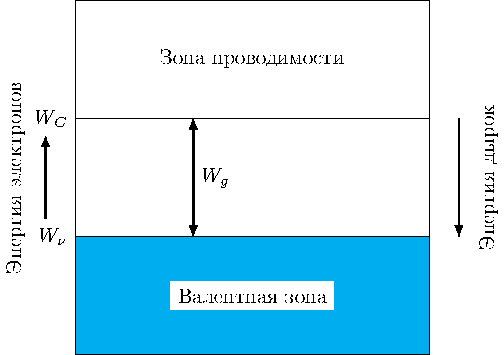
\includegraphics[width = \linewidth]{img/cond.pdf}
		\caption{Энергитический спектр электрона в кристалле. $W_c,W_{\nu}$ - соответственно, энергии дна зоны проводимости и потолка валентной зоны, $W_g$ - ширина запрещенной зоны.}
		\label{fig:cond}
	\end{wrapfigure}
	
	Представление о разрешенных и запрещенных зонах в сочетании с принципом Паули позволяет понять причину глубокого
	различия физических свойств металлов, диэлектриков и полупроводников. Действительно, если при абсолютном нуле зона
	проводимости полупроводника частично заполнена электронами или имеется перекрытие заполненной валентной зоны и пустой
	зоны проводимости, то в случае приложения электрического поля будут осуществляться энергетические переходы,
	обусловленные ускорением электронов во внешнем поле. Такие материалы проводят электрический ток даже при абсолютном нуле
	температуры и являются металлами.  
	
	Теперь рассмотрим ситуацию, когда между валентной зоной и зоной проводимости имеется запрещенная зона конечной ширины
	(рис. \ref{fig:cond}). В этом случае при абсолютном нуле, а также полном затемнении и не слишком сильном электрическом поле твердое
	тело не будет проводить электрический ток: в зоне проводимости электронов нет, а электроны заполненной валентной зоны не
	могут изменить своего состояния, поскольку все соседние уровни заняты. При повышении температуры и/или освещении такого
	тела электроны валентной зоны будут получать дополнительную энергию и переходить в зону проводимости. Вследствие таких
	переходов, во-первых, появятся электроны в зоне проводимости (они будут участвовать в переносе тока и обеспечивать
	электронную проводимость), а во-вторых, освободятся верхние уровни валентной зоны, что позволит и ее электронам
	участвовать в переносе тока, обеспечивая дырочную проводимость. Материал, имеющий запрещенную зону небольшой ширины,
	является полупроводником. Разница между полупроводниками и диэлектриками с точки зрения зонной теории заключается лишь в
	величине ширины запрещенной зоны.
	
	Ширина запрещенной зоны $W_g$  – один из важнейших параметров твердотельных материалов.
	При температуре 300 К она составляет в германии (Ge) 0.803 эВ, в кремнии (Si) – 1.12 эВ, в арсениде галлия (GaAs) – 1.43
	эВ, в фосфиде индия (InP) – 1.29 эВ.
	
	\subsection{Краткое описание кристаллической структуры полупроводников}
	Особенности энергетического спектра электронов в полупроводниках определяется кристаллическим строением твердых тел.
	Поэтому кратко остановимся написание кристаллической структуры полупроводников.
	
	Кристаллическую решётку определяет три базисных вектора $\vec{a},\vec{b},\vec{c}$ таких, что любая трансляция на вектор
	\begin{equation}
	\vec{R} = m \vec{a} + n \vec{b} + p \vec{c}
	\label{eq:1.1}
	\end{equation}
	представляющий собой линейную суперпозицию базисных векторов(m,n,p - произвольные целые числа), переводит
	кристаллическую решётку в саму себя. 
	
	Параллелепипед, построенный на базисных векторах, таким образом что его объем оказывается наименьшим по отношению к
	объемам параллелепипедов, построенным на всех прочих возможных комбинациях базисных векторов, получил название
	элементарной ячейки. Если элементарная ячейка содержит один атом, то такая ячейка называется простой и решетка,
	составленная из таких ячеек - простой. В случае когда элементарная ячейка содержит более одного атома говорят о сложной
	кристаллической решетке. В качестве примера на рис. \ref{fig:1.2} приведены решетки ряда химических элементов.
	
	\begin{figure}[h!]
		\centering
		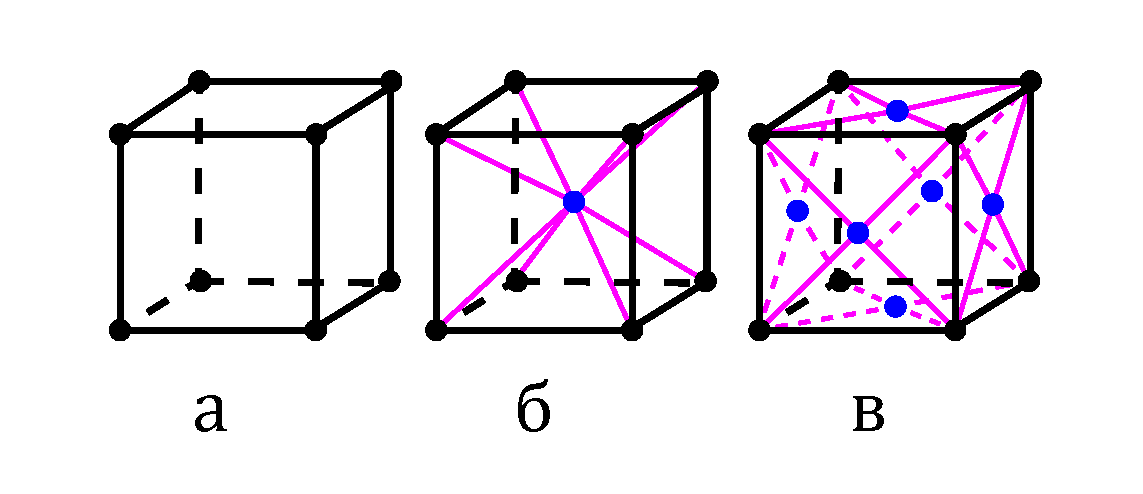
\includegraphics[width = .8\linewidth]{img/12}
		\caption{Простейшие типы элементарных ячеек кристаллов:(А) простая кубическая ячейка(Р); (Б) объемно-центрированная кубическая решетка (Na, W); (В) гранецентрированная кубическая ячейка (Al,Au)}
		\label{fig:1.2}
	\end{figure}
	
	Сложную решетку имеют широко используемые на практике полупроводники - кремний и германий (решетка типа алмаза) и
	GaAs(арсенид галлия)(решетка типа циковой обманки). Заметим, что решетка типа алмаза состоит из двух кубических
	гранецентрированных решеток атомов (см. рис. \ref{fig:1.2}) одного сорта, сдвинутых одна относительно другой на четверть
	пространственной диагонали; решетка типа цинковой
	\href{https://ru.wikipedia.org/wiki/%D0%9E%D0%B1%D0%BC%D0%B0%D0%BD%D0%BA%D0%B8}{обманки} такая же, только каждая из двух
		подрешеток состоит из атомов своего сорта.
		
		Положение атомных плоскостей и направления в кристаллической решетке определяют индексами Миллера. Прямая, определяемая
		индексами h,k,l (обозначается [hkl]) проходит из начала координат O в точку A, определяемую вектором $h \vec{a} + k
		\vec{b} + l \vec{c}$. В качестве примера заметим, что комбинация [100] характеризует направление вдоль оси Ox.
		Совокупность всех эквивалентных направлений обозначается <hkl>. Для описания положения плоскости нужно сначала найти точки, в которых рассматриваемая
		плоскость пересекает координатные оси, и записать их в единицах постоянных решетки, а затем взять обратные значения
		полученных целых чисел и привести их к наименьшему целому, кратному каждому из этих значений. Полученный результат
		заключают в круглые скобки (hkl). Это и есть индексы Миллера отдельной плоскости или семейства параллельных плоскостей.
		На рис. \ref{fig:1.3} показаны основные плоскости кубического кристалла и соответствующие индексы Миллера
		
		\begin{figure}[h!]
			\centering
			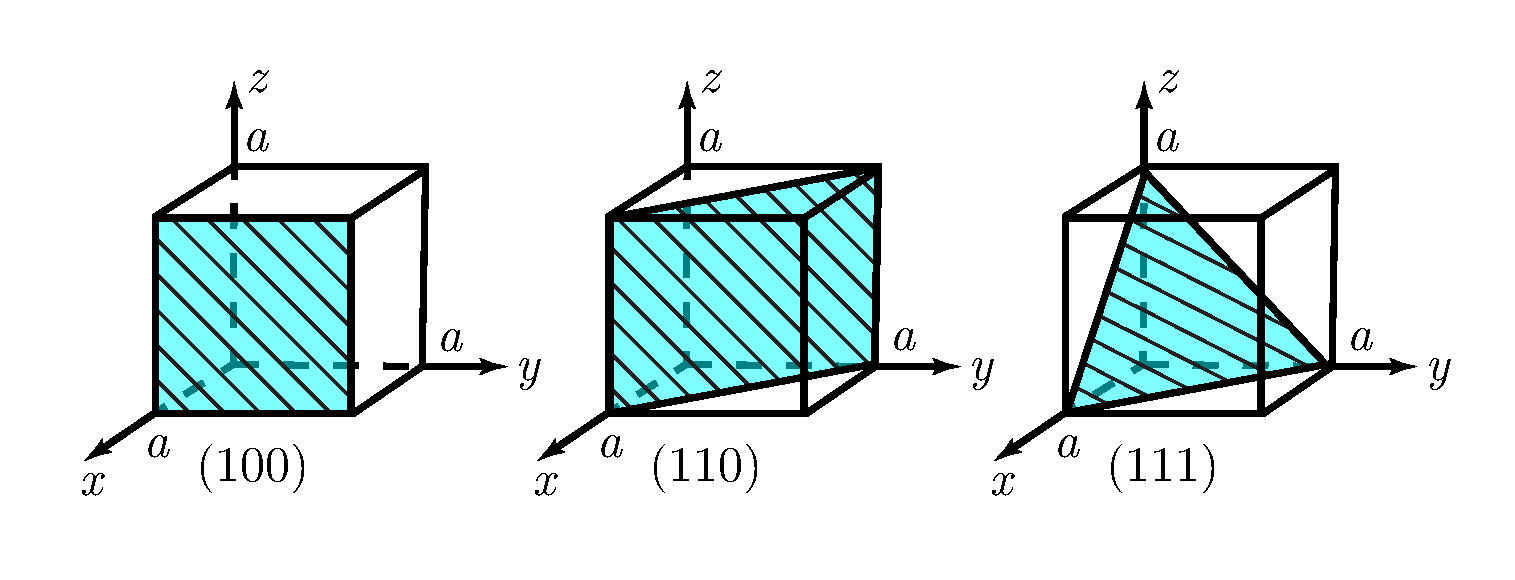
\includegraphics[width = .8\linewidth]{img/13}
			\caption{Индексы Миллера основных плоскостей кубического кристалла}
			\label{fig:1.3}
		\end{figure}
		
		В ряде случаев (например, при анализе движения электронов в кристалле) удобно использовать понятие обратной решетки.
		Базисные векторы обратной решетки $\vec{a}^*,\vec{b}^*,\vec{c}^*$ определяются на основании набора базисных векторов
		прямой решетки $\vec{a},\vec{b},\vec{c}$ с помощью соотношений
		\begin{equation}
		\vec{a}^{*}=2 \pi \frac{[\vec{b}, \vec{c}]}{(\vec{a}, [ \vec{b}, \vec{c}])}, \vec{b}^{*}=2 \pi \frac{[\vec{c}, a]}{(a,[\vec{b}, \vec{c}])}, \vec{c}^{*}=2 \pi \frac{[\vec{a}, \vec{b}]}{(\vec{a},[\vec{b}, \vec{c}])}
		\label{eq:1.2}
		\end{equation}
		
		При этом они обладают свойствами, которые мы сформулируем для вектора обратной решетки $\vec{a}^{*} :\left(\vec{a}^{*},
		\vec{a}\right)=2 \pi; \left(\vec{a}^{*}, \vec{b}\right)=0 ;\left(\vec{a}^{*}, \vec{c}\right)=0$. Аналогичными свойствами
		обладают также вектора $\vec{b}^{*},\vec{c}^{*}$.
		Произвольный вектор обратной решетки имеет вид:
		\begin{equation}
		\vec{G}=h \vec{a}^{*}+k \vec{b}^{*}+l \vec{c}^{*}
		\label{eq:1.3}
		\end{equation}
		где h,k,l - целые числа. Отсюда следует, что скалярное произведение $\vec{G} \cdot \vec{R}=2 \pi \cdot C$ (где C - целое
		число). Таким образом, любой вектор обратной решетки перпендикулярен соответствующим плоскостям прямой решетки, а объем
		элементарной ячейки обратной решетки обратно пропорционален объему элементарной ячейки прямой решетки, т.е. $V_{c}^{*}=(2 \pi)^{3}/V_{c},$ где $V_{c}=(a,[\vec{b}, \vec{c}])$
		
		Выбор элементарной ячейки как в пространстве прямой, так и в пространстве обратной решетки не является однозначным.
		Элементарную ячейку можно построить, пользуясь способом, предложенным Дирихле. А именно, для ее построения надо провести
		перпендикулярные плоскости через середины отрезков, соединяющих выбранный узел кристаллической решетки с ближайшими
		эквивалентными узлами. Образующаяся в результате этого построения элементарная ячейка в пространстве обратной решетки
		получила название ячейки Вигнера Зейтца.
		
		Используя построение Дирихле можно построить элементарную ячейку для объемно-центрированной кубической решетки. Для
		этого сначала проводятся отрезки из центральной точки куба ($\Gamma$) ко всем восьми его вершинам, а затем через середины этих
		отрезков проводятся соответствующие перпендикулярные плоскости; в конечном итоге получается усеченный тетраэдр внутри
		куба \ref{fig:1.4}, который и является элементарной ячейкой.
		\begin{figure}[h!]
			\centering
			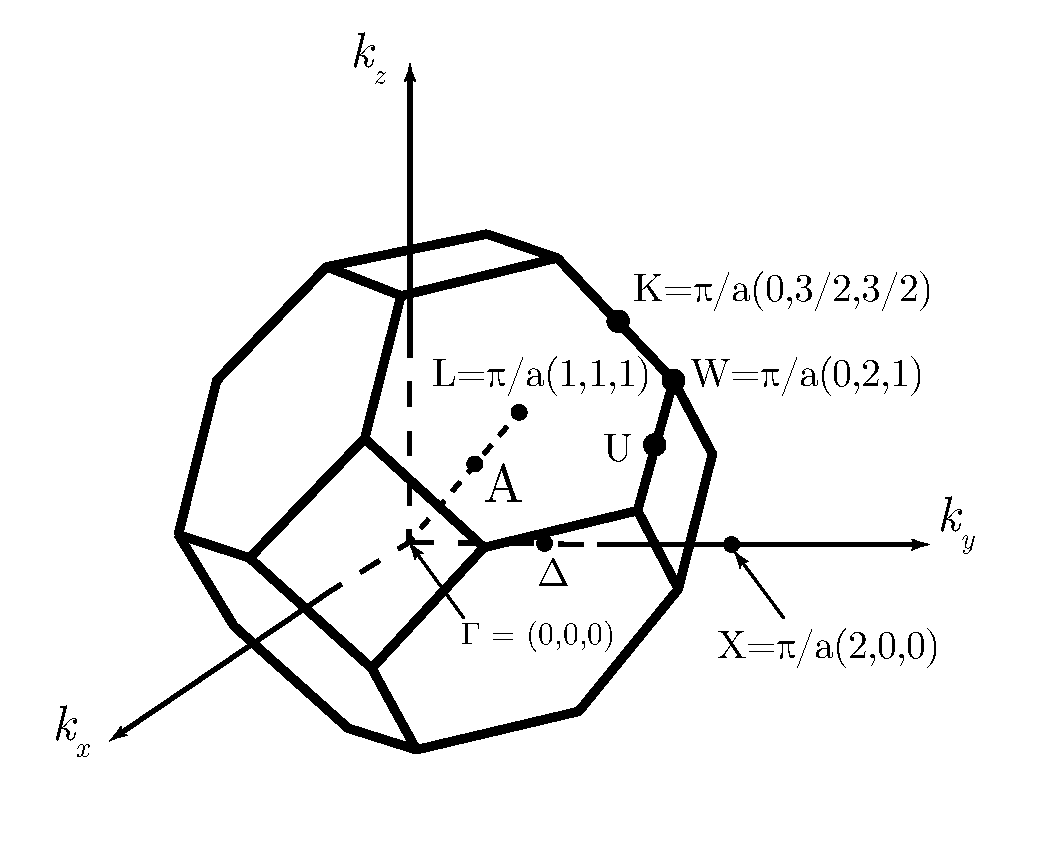
\includegraphics[width = .8\linewidth]{img/14}
			\caption{Ячейка Вигнера-Зейтца для гранецентрированной кубической решетки кристалла}
			\label{fig:1.4}
		\end{figure}
		С другой стороны, можно показать, что для гранецентрированной кубической прямой решетки с постоянной $a$ обратной является
		объемно-центрированная кубическая решетка с-постоянной $4 \pi /a$. Следовательно, показанная на рис.\ref{fig:1.4} элементарная ячейка
		является ячейкой Вигнера — Зейтца обратной решетки, соответствующей прямой гранецентрированной кубической решетке.
		
		Нахождение энергетического спектра электронов в разрешенной зоне в одноэлектронном приближении требует решения одночастичного уравнения Шредингера
		\begin{equation}
		\left[-\frac{\hbar^{2}}{2 m} \Delta+V(\vec{r})\right] \psi(r)=W \psi(\vec{r})
		\label{eq:1.4}
		\end{equation}
		где $\psi(\vec{r})$ - волновая функция электрона, m - его масса, W собственные значения квантовомеханического оператора
		энергии, заключенного в скобках. Поскольку потенциал $V(\vec{r})$ в кристалле периодически зависит от координат (с
		пространственным периодом, соответствующим постоянной решетки), то, согласно теореме Блоха, решения уравнения
		\eqref{eq:1.2} имеют вид
		\begin{equation}
		\psi_{k}(\vec{r})=e^{i(\vec{k}, \vec{r})} U_{\vec{k}}(\vec{r})
		\label{eq:1.5}
		\end{equation}
		где $ U_{\vec{k}}$ - периодические функции координат с периодом прямой решетки в соответствующей разрешенной зоне,
		$\vec{k}$ - вектор, характеризующий квантовое состояние электрона в кристалле, имеющий размерность волнового вектора и
		поэтому названный квазиволновым вектором. Функции называют блоховскими функциями. Можно ввести понятие квазиимпульса
		электрона с помощью соотношения $\vec{p}=\hbar \vec{k}$.
		
		Квазиволновой вектор электрона обладает свойством неоднозначности. Согласно зонной теории, в идеальной кристаллической
		решётке он определён с точностью до вектора обратной решетки. Это обстоятельство позволяет ограничить изменение
		компонент квазиволнового вектора конечной областью, исчерпывающей все физически неэквивалентные их значения. Область,
		включающая совокупность всех физически неэквивалентных значений квазиволнового вектора, называется зоной Бршлюэна.
		Вообще говоря, выбор зоны Бриллюэна содержит некоторый элемент произвола. Зачастую в качестве зоны Бриллюэна выбирают
		область, определяемую неравенствами
		\begin{equation}
		\left\{\begin{array}{l}{-\pi<(\vec{k}, \vec{a})<\pi} \\ {-\pi<(\vec{k}, \vec{b})<\pi} \\ {-\pi<(\vec{k}, \vec{c})<\pi}\end{array}\right.
		\label{eq:1.6}
		\end{equation}
		Эти неравенства определяют некоторую область в пространстве квазиволновых векторов, содержащую в себе начало координат.
		Эту область называют первой зоной Бриллюэна. Она представляет из себя ничто иное как ячейку Вигнера-Зейтца. Первая зона
		Бриллюэна для решеток алмаза и цинковой обманки (т е. для полупроводников Si, Ge, GaAs и ряда других) показана на рис.
		\ref{fig:1.4}, где также отмечены главные точки и линии симметрии.
		
		Остановимся теперь на свойствах функции, описывающей энергию электронов в разрешенной зоне $(W=W(\vec{k}))$ от квазиволнового
		вектора. Из теоремы Блоха следует, что энергия электрона в разрешенной зоне является функцией квазиволнового вектора $\vec{k}$,
		т.е. $W=W(\vec{k})$, обладающей свойством периодичности с периодом, равным вектору обратной решетки. Зонные энергетические
		спектры рассчитываются теоретически с помощью различных приближенных методов.
		
		Существуют несколько способов изображения энергии как функции $\vec{k}$. Самый простой - это графическое изображение $W=W(\vec{k})$ в
		виде дисперсионных кривых для некоторых выбранных направлений. Дисперсионные кривые для Si, Ge и GaAs показаны на рис.
		\ref{fig:1.5}. Заметим только, что зона проводимости основных полупроводников состоит из нескольких подзон (или долин, областей в
		окрестности экстремумов зависимости  $W(\vec{k})$) (рис. \ref{fig:1.5}). Так, в Ge имеется 8 эквивалентных долин на осях <111>, в Si — 6 на
		осях <100>, а в GaAs дно зоны проводимости находится при к=0, Валентная зона в кристаллах со структурой цинковой обманки
		состоит из четырех подзон (если пренебречь спином в уравнении Шредингера), двукратно вырожденных по спину. Три из них
		вырождены в центре зоны k=0 ($\Gamma$ - точка) и формируют верхний край валентной зоны, а четвертая подзона образует ее дно.
		Спин-орбитальное взаимодействие частично снимает вырождение при к=0 и приводит к отщеплению одной подзоны, как видно из
		рис. \ref{fig:1.5}. Полупроводники, в которых дно зоны проводимости и потолок валентной зоны располагаются в одной и той же точке
		зоны Бриллюэна (GaAs) называются прямозонными. В противном случае проводники называются непрямозонными (Ge, Si).
		
		\begin{figure}[h!]
			\centering
			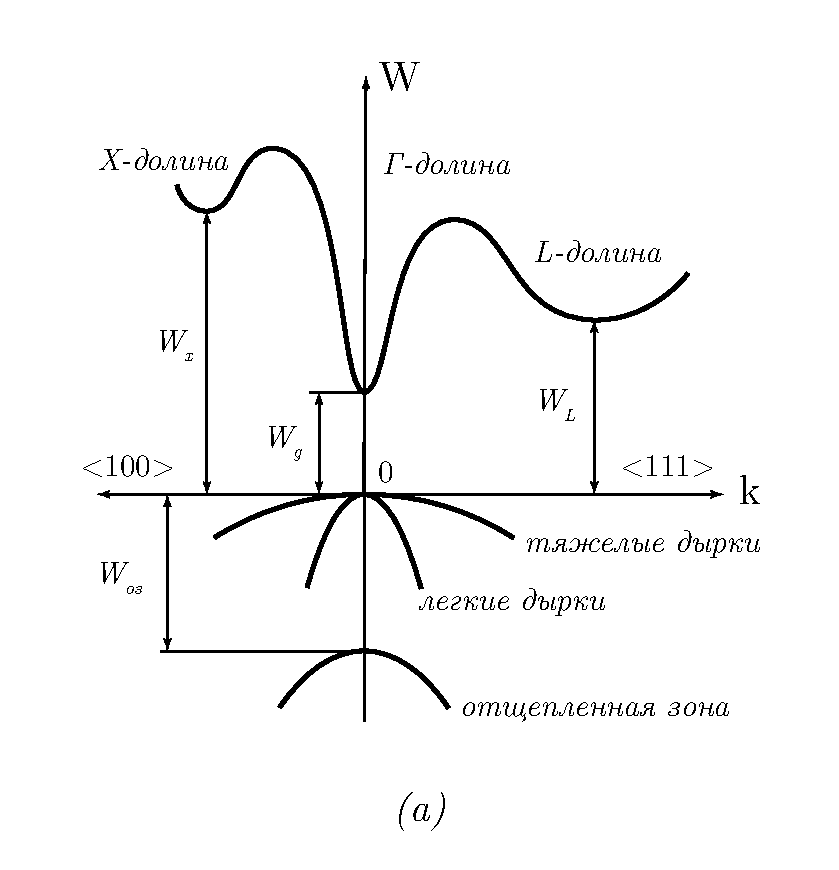
\includegraphics[width = .45\linewidth]{img/15a}
			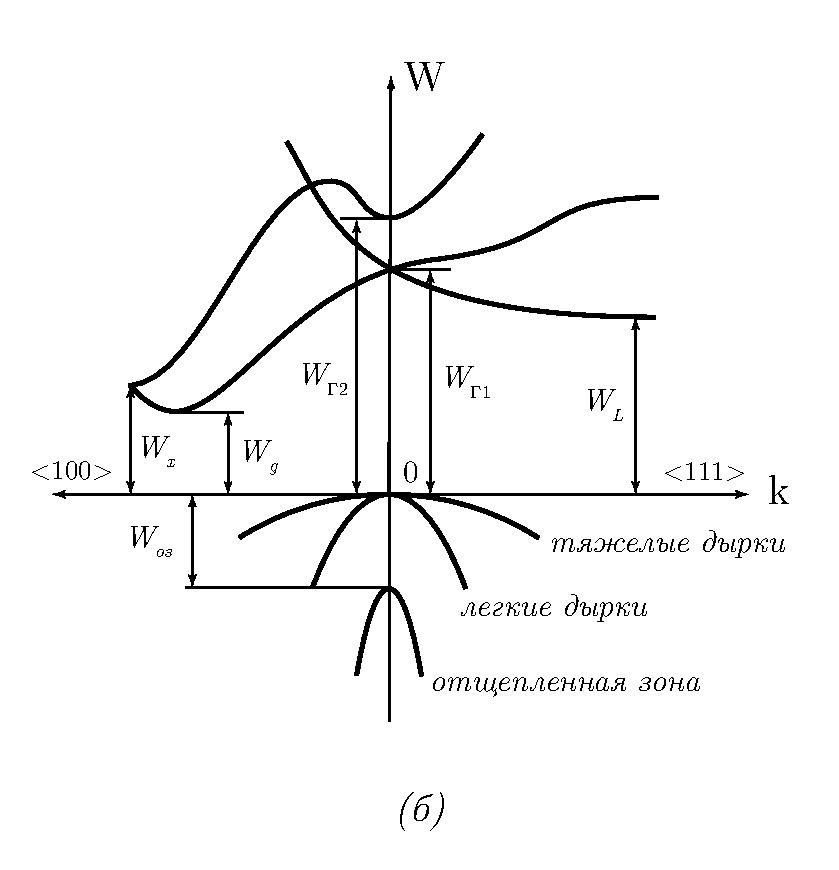
\includegraphics[width = .45\linewidth]{img/15b}
			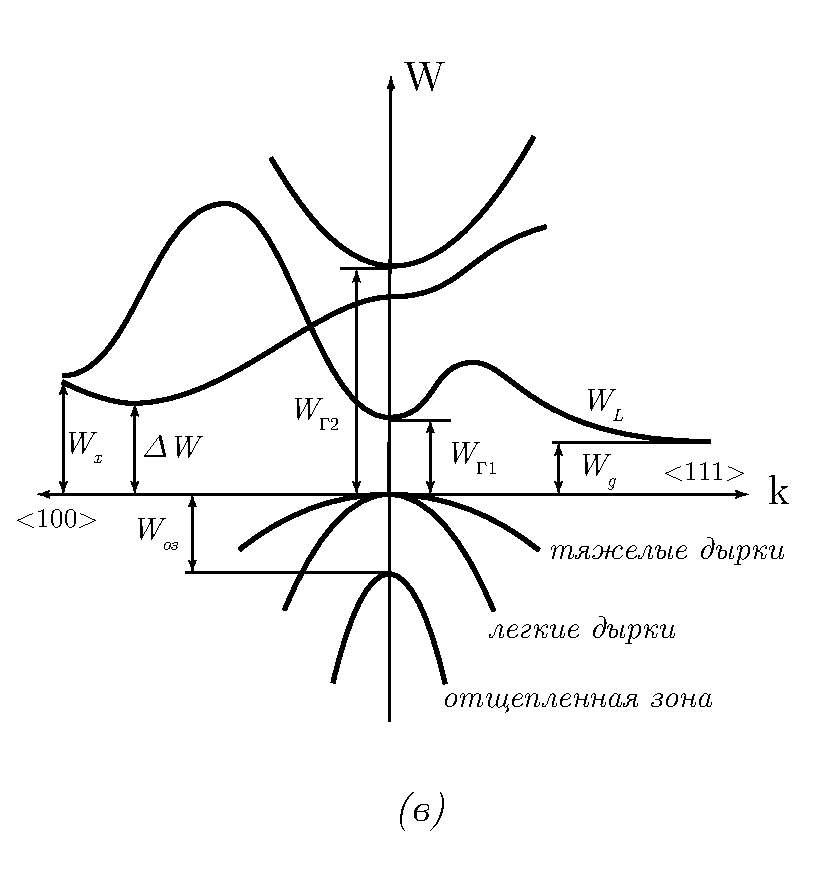
\includegraphics[width = .45\linewidth]{img/15v}
			\caption{Структура энергетических зон полупроводниковых материалов: (a) GaAs; (б) Si; (в) Ge}
			\label{fig:1.5}
		\end{figure}
		
		Другой возможный способ графического представления $W=W(\vec{k})$ это изображение поверхностей постоянной энергии
		(изоэнергетических поверхностей). Примеры изоэнергетических поверхностей для электронов в зоне проводимости в Si, Ge и
		GaAs приведены на рис. \ref{fig:1.6}. В частности, видно, что в Si и Ge изоэнергетическими поверхностями являются эллипсоиды. В Ge
		границы зоны Бриллюэна проходят точно посередине эллипсоидов, так что от каждого из них в первой зоне Бриллюэна остается
		половина (четыре полных эллипсоида в зоне Бриллюэна), и, следовательно, эти поверхности постоянной энергии центрированы
		в L-точке. В Si имеется 6 эквивалентных эллипсоидов, центрированных на осях <100> на расстоянии от центра зоны, равном
		примерно $\frac{3}{4}$ полной длины соответствующей оси. В GaAs изоэнергетическими поверхностями являются сферы с центром в середине
		зоны Бриллюэна.
		
		\begin{figure}[h!]
			\centering
			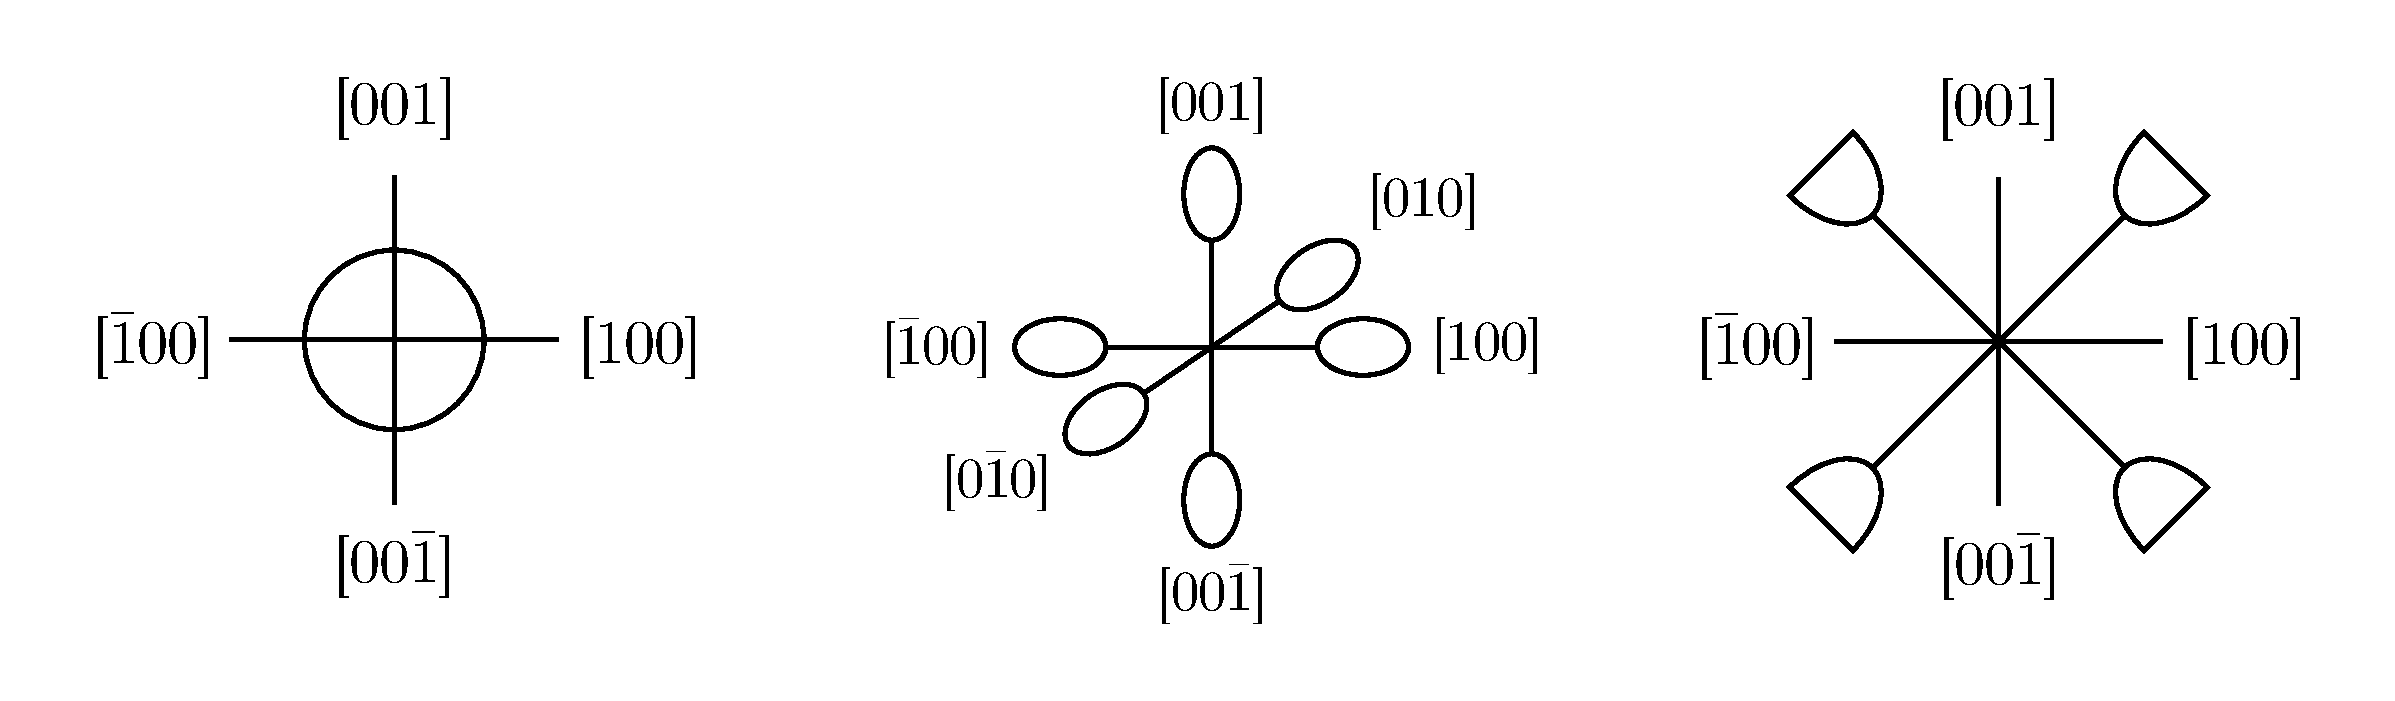
\includegraphics[width = .95\linewidth]{img/16}
			\caption{Сечения поверхностей постоянной энергии для электронов в зоне проводимости: (a) GaAs; (б) Si; (в) Ge}
			\label{fig:1.6}
		\end{figure}
		
		Несмотря на сложность зависимости энергии электрона от квазиволнового вектора в большинстве задач физики полупроводников
		играет роль поведение электрона в достаточно узкой области значений квазиволнового вектора в зоне Бриллюэна вблизи
		минимума или максимума энергии. Вблизи точки экстремума $\vec{k}_0$ функцию $W=W(\vec{k})$ можно разложить в ряд Тейлора, используя
		выражение
		
		\begin{equation}
		W(\vec{k})=W\left(\vec{k}_{0}\right)+\frac{1}{2} \sum_{i=x}^{z} \sum_{j=x}^{z} \frac{1}{m_{i j}^*} \hbar^{2}\left(k_{i}-k_{i 0}\right)\left(k_{j}-k_{j 0}\right)
		\label{eq:1.7}
		\end{equation}
		
		где $m_{i j}^*$ - эффективная масса носителей заряда, являющаяся тензором, компоненты которого определяются соотношением
		\begin{equation}
		\frac{1}{m^{*}_{i j}}=\frac{1}{\hbar^{2}} \frac{\partial^{2} W(k)}{\partial k_{i} \partial k_{j}}
		\label{eq:1.8}
		\end{equation}
		Эффективная масса характеризует взаимодействие носителей заряда с идеальной кристаллической решеткой.
		
		\section{Концентрация носителей заряда в полупроводнике}
		Вычисление концентрации подвижных и связанных носителей заряда в полупроводнике составляет задачу статистики электронов.
		Решение этой задачи, с одной стороны, позволяет объяснить экспериментальные результаты, по которым, в свою очередь,
		становится возможным определение ряда важных характеристик полупроводника (ширины запрещенной зоны, энергия ионизации примеси).
		Задача вычисления концентрации носителей заряда распадается на две:  1) определение числа возможных квантовых состояний
		электронов в разрешенных зонах в твердом теле и 2) выяснение фактического распределения электронов по этим квантовым
		состояниям. Рассмотрим последовательно решение каждой из подзадач.
		
		Число состояний в любой зоне кристалла равно общему числу мест на уровнях изолированных атомов, образовавших кристалл,
		т.е. числу атомов $N_0$, умноженному на кратность вырождения $\nu$ атомного уровня, образовавшего данную зону:
		
		\begin{equation}
		\int \limits_{W_1}^{W_2} N(W) dW  =\nu N_0 
		\label{eq:2.1}
		\end{equation} 
		
		где $N(W)dW$ - число  квантовых состояний в интервале энергий от $W$ до $W+dW$ в единице объёма полупроводника, а $N(W)$
		-  плотность квантовых состояний. $W_1,W_2$ - энергии нижнего и верхнего края зоны, соответственно. 
		
		Нахождение точного вида функции $N(W)$ – очень сложная задача. Приведем ее решение для простейшего случая, когда электроны
		заполняют только уровни вблизи дна зоны проводимости, т.е. для описания зависимости энергии носителей от квазиимпульса
		$W(~\vec{p}~)$ справедливо приближение эффективной массы:   
		\begin{equation}
		W = W_C + \frac{p^2}{2m_n^*}
		\label{eq:2.2}
		\end{equation}
		
		где $W_C$ – энергия дна зоны проводимости, $m_n^*$ –  эффективная масса электрона на дне зоны проводимости, $\vec{p} =
		\hbar \vec{k}$ – квазиимпульс электрона, $\vec{k}$ – квазиволновой вектор. Число состояний в интервале энергий $(W, W+dW)$ может быть найдено
		путем определения отношения объема в пространстве квазиволновых векторов (kпространстве), заключенного между двумя
		указанными изоэнергетическими поверхностями, к объему одного квантового состояния. 
		
		В случае закона дисперсии, представленного в виде \eqref{eq:2.2} поверхности равной энергии в k-пространстве являются
		сферами с радиусом k. Выделим шаровой слой, заключенный между двумя изоэнергетическими поверхностями, соответствующими
		энергиям $W$ и $W+dW$. Объем этого слоя имеет величину: 
		\begin{equation}
		dV_p = 4 \pi k^2 d k
		\label{eq:2.3}
		\end{equation}
		Объём, приходящийся на одно электронное состояние равен $dk_x dk_y dk_z = \frac{(2 \pi)^3}{V}$ , где $V$ – объём
		кристалла. В каждой ячейке могут находиться два электрона с противоположными спинами. С учетом этого, число состояний в
		объеме $dV_p$ равно: 
		\begin{equation}
		d Z=2 \frac{d V_{p}}{(2 \pi \hbar)^{3}}=\frac{k^{2} d k}{\pi^{2}}
		\label{eq:2.4}
		\end{equation}
		Из равенства \eqref{eq:2.2} получаем: 
		\begin{equation}
		\hbar k=\sqrt{2 m_{n}^{*}\left(W-W_{C}\right)}
		\label{eq:2.5}
		\end{equation}
		откуда:
		\begin{equation}
		d k=\frac{1}{2 \hbar}\left(2 m_{n}^{*}\left(W-W_{C}\right)\right)^{-1 / 2} d W
		\label{eq:2.6}
		\end{equation}
		Подставляя \eqref{eq:2.5} и \eqref{eq:2.6} в \eqref{eq:2.4}, получим выражение для плотности квантовых состояний у дна зоны
		проводимости:
		\begin{equation}
		N_{c}(W)=\frac{d Z}{d W}=4 \pi\left[\frac{2 m_{n}^{*}}{(2 \pi \hbar)^{2}}\right]^{3 / 2} \sqrt{W-W_{C}}
		\label{eq:2.7}
		\end{equation} 
		Аналогично определяется плотность состояний вблизи потолка валентной зоны.
		
		Для определения числа электронов в зоне проводимости или дырок в валентной зоне кроме плотности состояний необходимо
		знать также вероятность заполнения каждого состояния (уровня энергии) электронами. Если считать электроны
		невзаимодействующими, как это обычно делается, то газ электронов подчиняется законам идеального газа. 
		
		Статистическое описание электронов основано на следующих двух свойствах. Во-первых это неразличимость электронов,
		протекающая в квантовой механике из расплывание волновых пакетов, и во-вторых, принцип Паули, запрещающий двум
		электронным находиться в одном квантовом состоянии. Статистика электронов подчиняется распределение Ферми-Дирака:   
		\begin{equation}
		f(W) = \frac{1}{\exp(\frac{W-W_F}{k_B T})+1}
		\label{eq:2.8}
		\end{equation}
		которое даёт вероятность того, что в тепловом равновесии состояние с энергией $W$ занято электроном. Здесь $k_B$ –
		постоянная Больцмана, $Т$ – абсолютная температура, $W_F$ – энергия (уровень) Ферми – максимальная энергия электронов при
		абсолютном нуле. Для температуры, отличной от нуля, функция $f(W)$ в точке $W = W_F$ имеет перегиб.
		
		Рассмотрим случай, когда $T > 0$. Из выражения \eqref{eq:2.8} следует, что для $W=W_F: f(W) =1/2$. При очень больших энергиях, когда 
		$ W-W_F>> k_B T $, можно пренебречь 1 в знаменателе, и выражение $f(W)$ принимает вид:
		\begin{equation}
		f(W) = \exp(\frac{W_F-W}{k_B T})
		\label{eq:2.9}
		\end{equation} 
		т.е. совпадает с функцией Максвелла-Больцмана для частиц, подчиняющихся классическим законам. Аналогично, при очень
		малых энергиях, когда $W<<W_F$ (но $W-W_F>>k_B T$), экспонента в знаменателе \eqref{eq:2.8} очень мала и, разлагая функцию $f(W)$ в ряд по
		малому параметру и ограничиваясь нулевым и первым слагаемыми, получим: 
		\begin{equation}
		f(W) = 1 - \exp( \frac{W-W_F}{k_BT})
		\label{eq:2.10}
		\end{equation}
		Зависимость плотности состояний в зоне проводимости от энергии и вероятности заполнения этих состояний позволяет
		определить концентрацию свободных электронов $dn$, энергия которых заключена в интервале от $W$ до $W+dW$:
		\begin{equation}
		dn = f(W) N(W)dW
		\label{eq:2.11}
		\end{equation}
		Интегрирование выражения \eqref{eq:2.11} по всей зоне проводимости позволяет найти полное число электронов в ней. Так как функция
		Ферми быстро спадает с ростом энергии, верхний предел можно заменить бесконечностью. 
		
		В элементарных функциях такой интеграл не вычисляется, и для его нахождения используют специальные таблицы. Однако, если
		уровень Ферми лежит в запрещенной зоне достаточно далеко от ее краев, т.е. $W_c - W_F>>k_B T$ , то для функции Ферми
		справедливо приближение Больцмана и интеграл можно вычислить. Такой полупроводник называется невырожденным. Интегрируя
		\eqref{eq:2.11} в данном приближении, получим: 
		\begin{equation}
		n=\int_{W_{C}}^{\infty} f(W) N(W) d W=N_{c} \exp(-\frac{W_C-W_F}{k_B T})
		\label{eq:2.12}
		\end{equation}
		где $N_{c}=2\left[\frac{2 \pi m_{n}^{*} k_{B} T}{h^{2}}\right]^{3 / 2}$ - эффективная плотность состояний в зоне проводи
		мости.
		
		Аналогично концентрация дырок: 
		\begin{equation}
		p=N_{\nu} e^{-\frac{W_{F}-W_{\nu}}{k_{B} T}}
		\label{eq:2.13}
		\end{equation}
		где $N_{\nu}=2\left[\frac{2 \pi m_{p}^{*} k_{B} T}{h^{2}}\right]^{3 / 2}$ - эффективная плотность состояний валентной зоне.
		
		Полученные выше выражения для концентрации электронов и дырок в совокупности с принципом электронейтральности
		полупроводника ( в однородном полупроводнике не может быть существенных нескомпенсированных объемных зарядов ни в
		равновесном состоянии, ни при наличии тока ) позволяют сделать выводы о положении уровня Ферми в полупроводнике.
		Рассмотрим собственный полупроводник, для которого влияние примесных атомов не существенно. Свободные носители заряда в
		этом случае возникают только за счет разрыва валентных связей. Поэтому в собственном полупроводнике концентрация дырок p
		равна концентрации электронов $ n: n = p \equiv n_i$. Это условие электронейтральности собственного полупроводника. Из этого
		условия, приравняв \eqref{eq:2.12} и \eqref{eq:2.12}, получим:
		\begin{equation}
		W_{F}=\frac{W_{c}+W_{v}}{2}+\frac{k_{B} T}{2} \ln \frac{N_{V}}{N_{c}}=\frac{W_{c}+W_{v}}{2}-\frac{3 k_{B} T}{4} \ln \frac{m_{n}^{*}}{m_{p}^{*}}
		\label{eq:2.14}
		\end{equation}
		т.е. уровень Ферми $W_F$ собственного полупроводника при абсолютном нуле температуры лежит в центре запрещенной зоны и,
		вообще говоря, смещается при возрастании температуры. Этот случай показан на рис.\ref{fig:2.1}(a), где слева направо схематически
		приведены простейшая зонная диаграмма, плотность состояний $N(W)$, распределение Ферми $f (W)$ и концентрация носителей
		заряда.
		
		
		\begin{figure}[h!]
			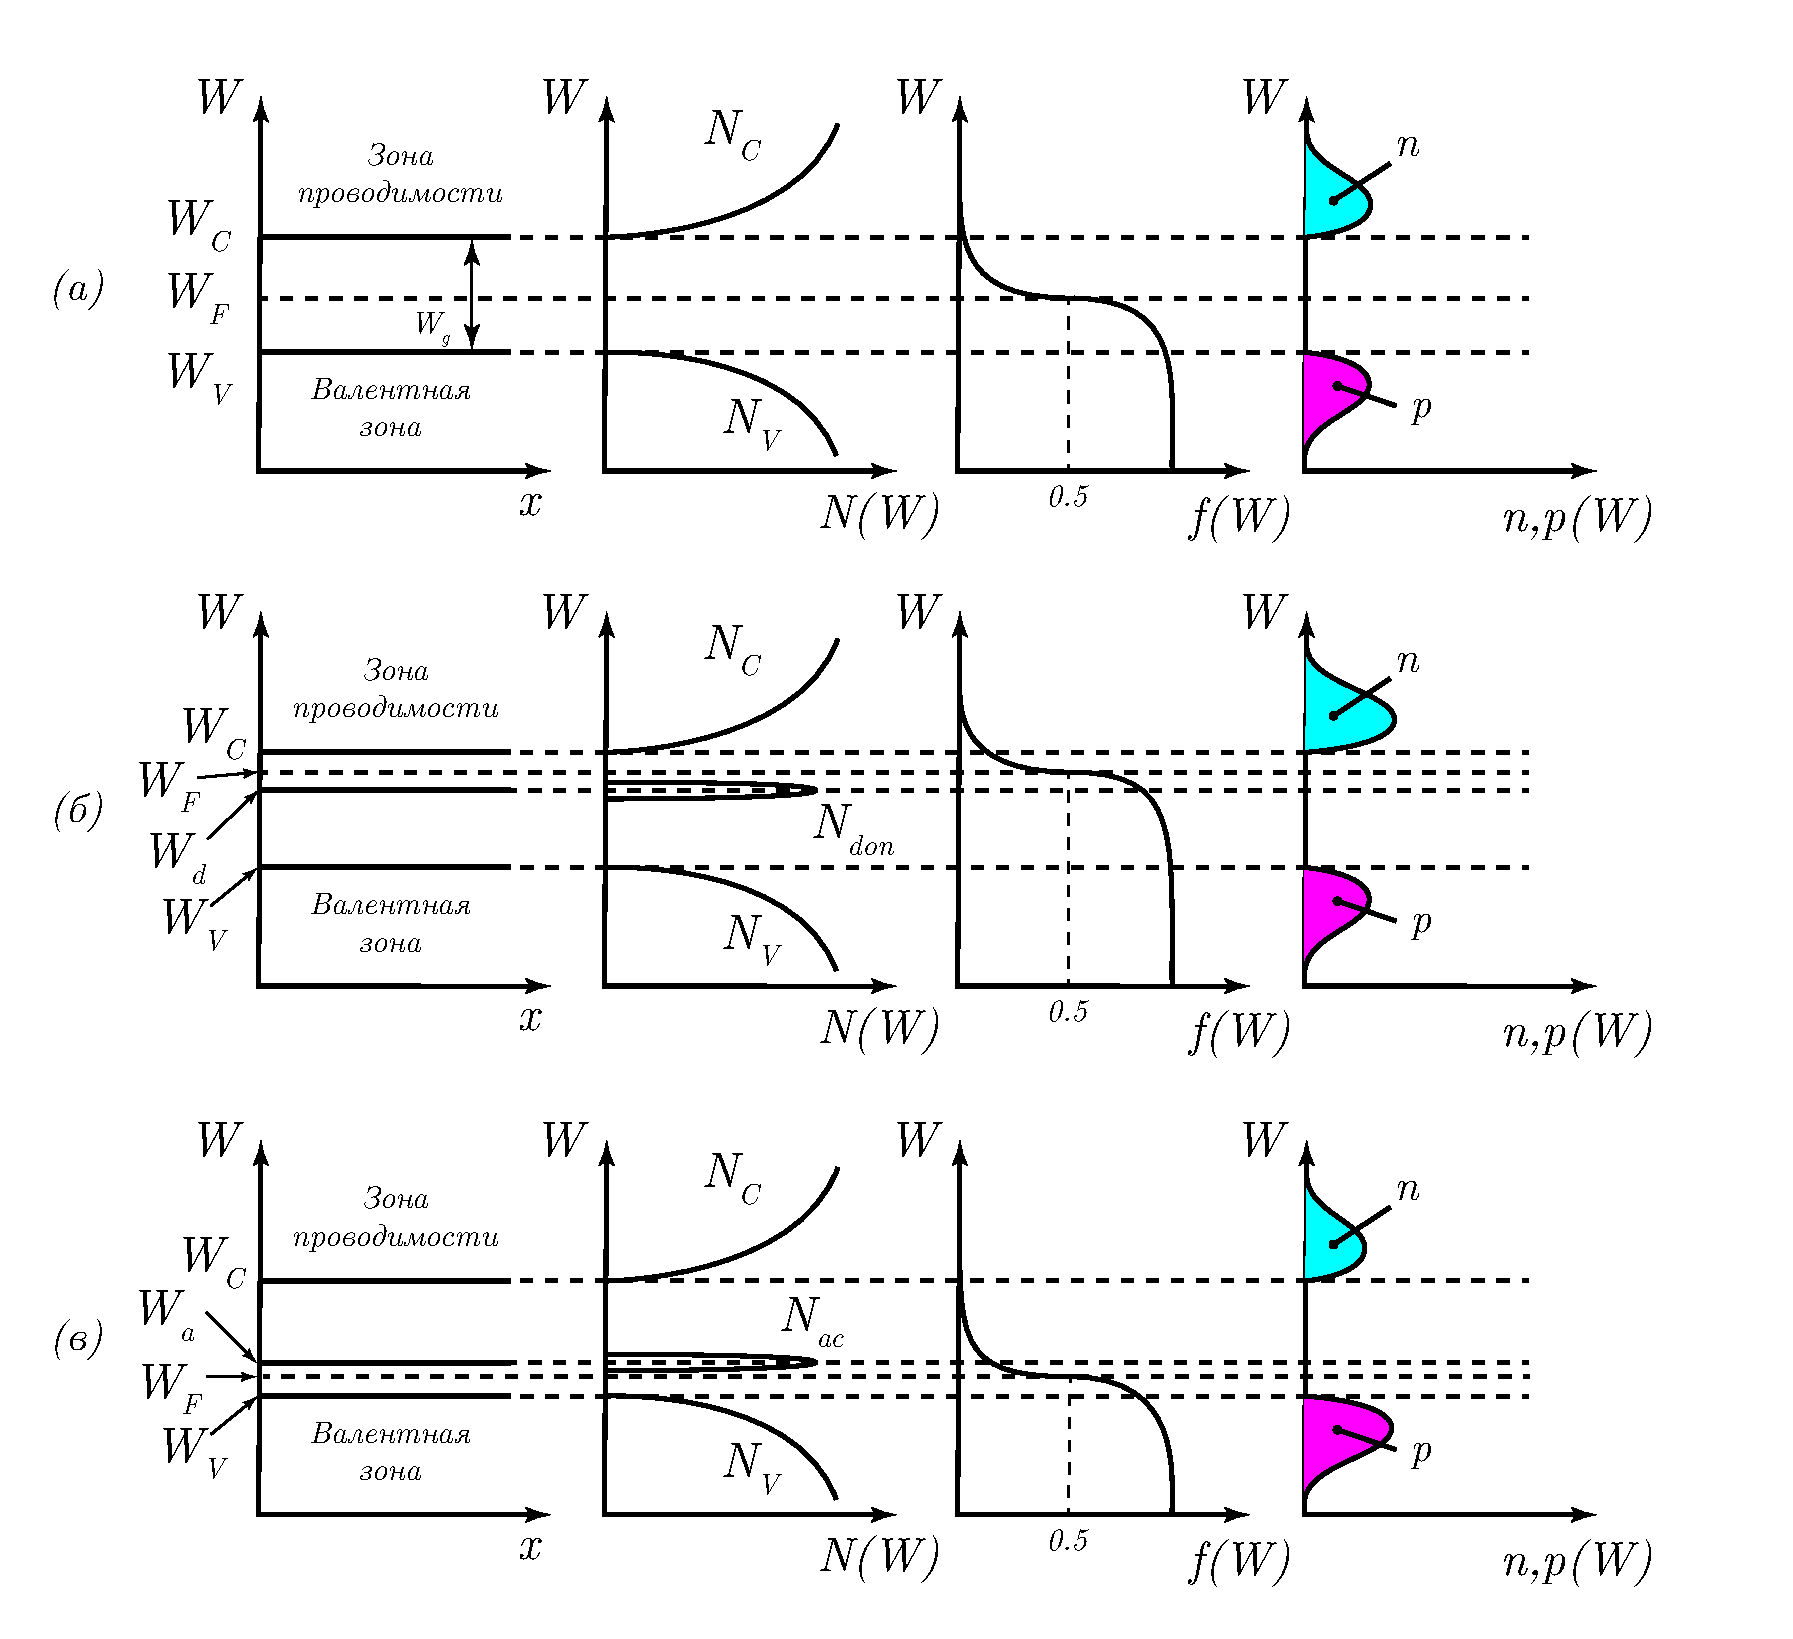
\includegraphics[width = \linewidth]{img/22}
			\caption{Графическое изображение решения уравнения электронейтральности для собственного полупроводника(а), для примесного полупроводника, легированного донорной (б) и акцепторной (в) примесью}
			\label{fig:2.1}
		\end{figure}
		
		Если в полупроводник введены примесные атомы, то, как показано на рис. \ref{fig:2.1}(б) и \ref{fig:2.1}(в), уровень Ферми должен смещаться для
		сохранения электронейтральности. В случае \ref{fig:2.1}(б), например, в кристалл добавляется донорная примесь, приводящая к
		образованию локальных энергетических уровней Wd. Пусть концентрация доноров составляет $N_d$ (см$^{-3}$). Для сохранения
		элентронейтральности отрицательный заряд электронов должен быть равен полному заряду дырок и ионизованных доноров:
		\begin{equation}
		n = N_d+p
		\label{eq:2.15}
		\end{equation}
		Следовательно, $n>р$ и уровень Ферми обязан сместиться к дну зоны проводимости, как показано на рис. \ref{fig:2.1}(б).
		
		Температурная зависимость концентраций электронов и дырок в собственном полупроводнике определяется формулами \eqref{eq:2.12} и \eqref{eq:2.13} с учетом
		\eqref{eq:2.14}. Этими же формулами определяются и концентрации носителей в примесном полупроводнике при достаточно высоких
		температурах, когда количество электронов в зоне проводимости и дырок в валентной зоне определяется переходами
		электронов через запрещенную зону. При этом уровень Ферми лежит вблизи середины запрещенной зоны, т.е. $W_F =
		\frac{W_c+W_{\nu}}{2}$. Подставляя последнее соотношение в \eqref{eq:2.12}, получим концентрацию электронов:
		\begin{equation}
		n=N_{c} e^{-\frac{W_{c}-W_{v}}{2 k_{B} T}}=N_{c} e^{-\frac{W_{g}}{2 k_{B} T}}
		\label{eq:2.16}
		\end{equation}
		где $W_g$  – ширина запрещенной зоны. Величина $N_c$ зависит от температуры по закону $Т^{3/2}$. Эта зависимость слабая по
		сравнению с экспонентой, поэтому температурная зависимость концентрации определяется, в основном, экспоненциальным
		множителем. 
		
		При низких температурах концентрация носителей в примесном полупроводнике определяется примесями. При очень низких
		температурах, когда еще не вся примесь ионизована, уровень Ферми, например, для электронного полупроводника, лежит
		примерно посередине между уровнем донорной примеси и дном зоны проводимости, т.е. $W_F = \frac{W_c+W_{d}}{2}$. Тогда \eqref{eq:2.12}
		принимает вид: 
		\begin{equation}
		n=N_{c} e^{-\frac{W_{c}-W_{d}}{2 k_{B} T}}=N_{c} e^{-\frac{\Delta W_{d}}{2 k_{B} T}}
		\label{eq:2.17}
		\end{equation}
		где $\Delta W_d$ – энергия ионизации донорной примеси. 
		
		Для более высоких температур, когда вся примесь ионизована, но вероятность перехода электронов из валентной зоны мала,
		концентрация носителей заряда просто равна концентрации примеси $n=N_d$. 
		
		
		Таким образом, зависимость концентрации от температуры имеет три участка (см. рис. \ref{fig:2.2}). Область примесной проводимости
		при низких температурах – 1-2; область истощения примесей – участок 2-3 и область собственной проводимости – участок
		3-4. В координатах $ln(n)$, $1/T$ экспоненты (2.16), (2.17.) выглядят как прямые, наклон которых характеризуется величинами
		$W_g$ и $\Delta W_d$. Результаты измерения температурной зависимости концентрации электронов позволяют определить ширину
		запрещенной зоны полупроводника и энергию ионизации примеси.
		
		\begin{figure}[h!]
			\centering
			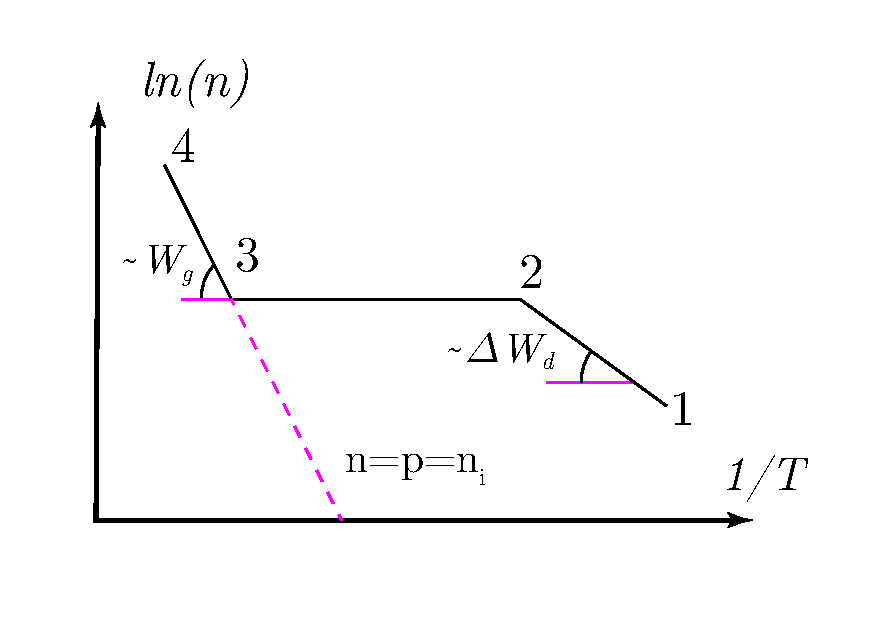
\includegraphics[width = .7\linewidth]{img/23}
			\caption{Зависимость концентрации носителей заряда от температуры в полупроводнике.}
			\label{fig:2.2}
		\end{figure}
		
		Измерение концентрации носителей заряда требует разработки специальной методики. Гораздо проще проводить измерения
		проводимости образца, но на нее, помимо концентрации носителей, оказывает влияние подвижность частиц. Поэтому далее мы
		разберем особенности движения носителей заряда в полупроводнике под действием электрического поля. 
		
		
		\section{Подвижность носителей заряда в полупроводнике}
		
		Движение электрона в кристалле под действием внешней силы F и сил со стороны кристаллической решетки в ряде случаев
		может быть описано как движение свободного электрона, на который действует только сила F (закон Ньютона), но с
		эффективной массой $m^*$, отличной от массы свободного электрона и в общем случае зависящей от энергии электрона. Это
		отличие отражает взаимодействие электрона проводимости с решеткой. 
		В реальной кристаллической структуре всегда присутствуют дефекты: тепловые колебания атомов решётки, примеси и т.д.
		Поэтому при воздействии внешнего электрического поля частица движется ускоренно лишь на небольшом участке пути, а затем
		испытывает рассеяние (взаимодействие с дефектами кристалла), изменяя свой импульс и ( в случае неупругого
		взаимодействия) энергию, теряет направленную скорость, после чего процесс разгона начинается заново (рис. \ref{fig:3.1}). В слабых
		электрических полях ($\leq 10^3$ В/см) средняя скорость направленного движения носителей заряда (дрейфовая скорость)
		пропорциональна напряжённости электрического поля:$\nu = \mu E$. Коэффициент пропорциональности между скоростью и полем $\mu$
		называется подвижностью носителей заряда. Эта величина численно равна средней скорости направленного движения частиц в
		электрическом поле с напряженностью 1 В/м. 
		
		Подвижность носителей заряда сильно меняется с изменением температуры. Для получения этой зависимости необходимо кратко
		остановится на основных механизмах рассеяния носителей заряда в полупроводниках. 
		
		Рассеяние носителей заряда на нейтральных атомах примеси и нейтральных дефектах является слабым. Однако, при низких
		температурах, когда примеси еще практически не ионизованы, а тепловые колебания отсутствуют, этот механизм играет
		существенную роль. Для того, чтобы электрон изменил направление своего движения в результате взаимодействия с
		нейтральной примесью или дефектом, необходимо, чтобы траектория электрона проходила через место расположения дефекта
		либо через примыкающую к нему область решетки, в которой им вызваны искажения. Рассеяние на нейтральных примесях не
		зависит от температуры, а подвижность, обусловленная этим рассеянием, постоянна и зависит только от концентрации
		рассеивающих центров.
		\begin{wrapfigure}{l}{0.3\linewidth}
			\centering
			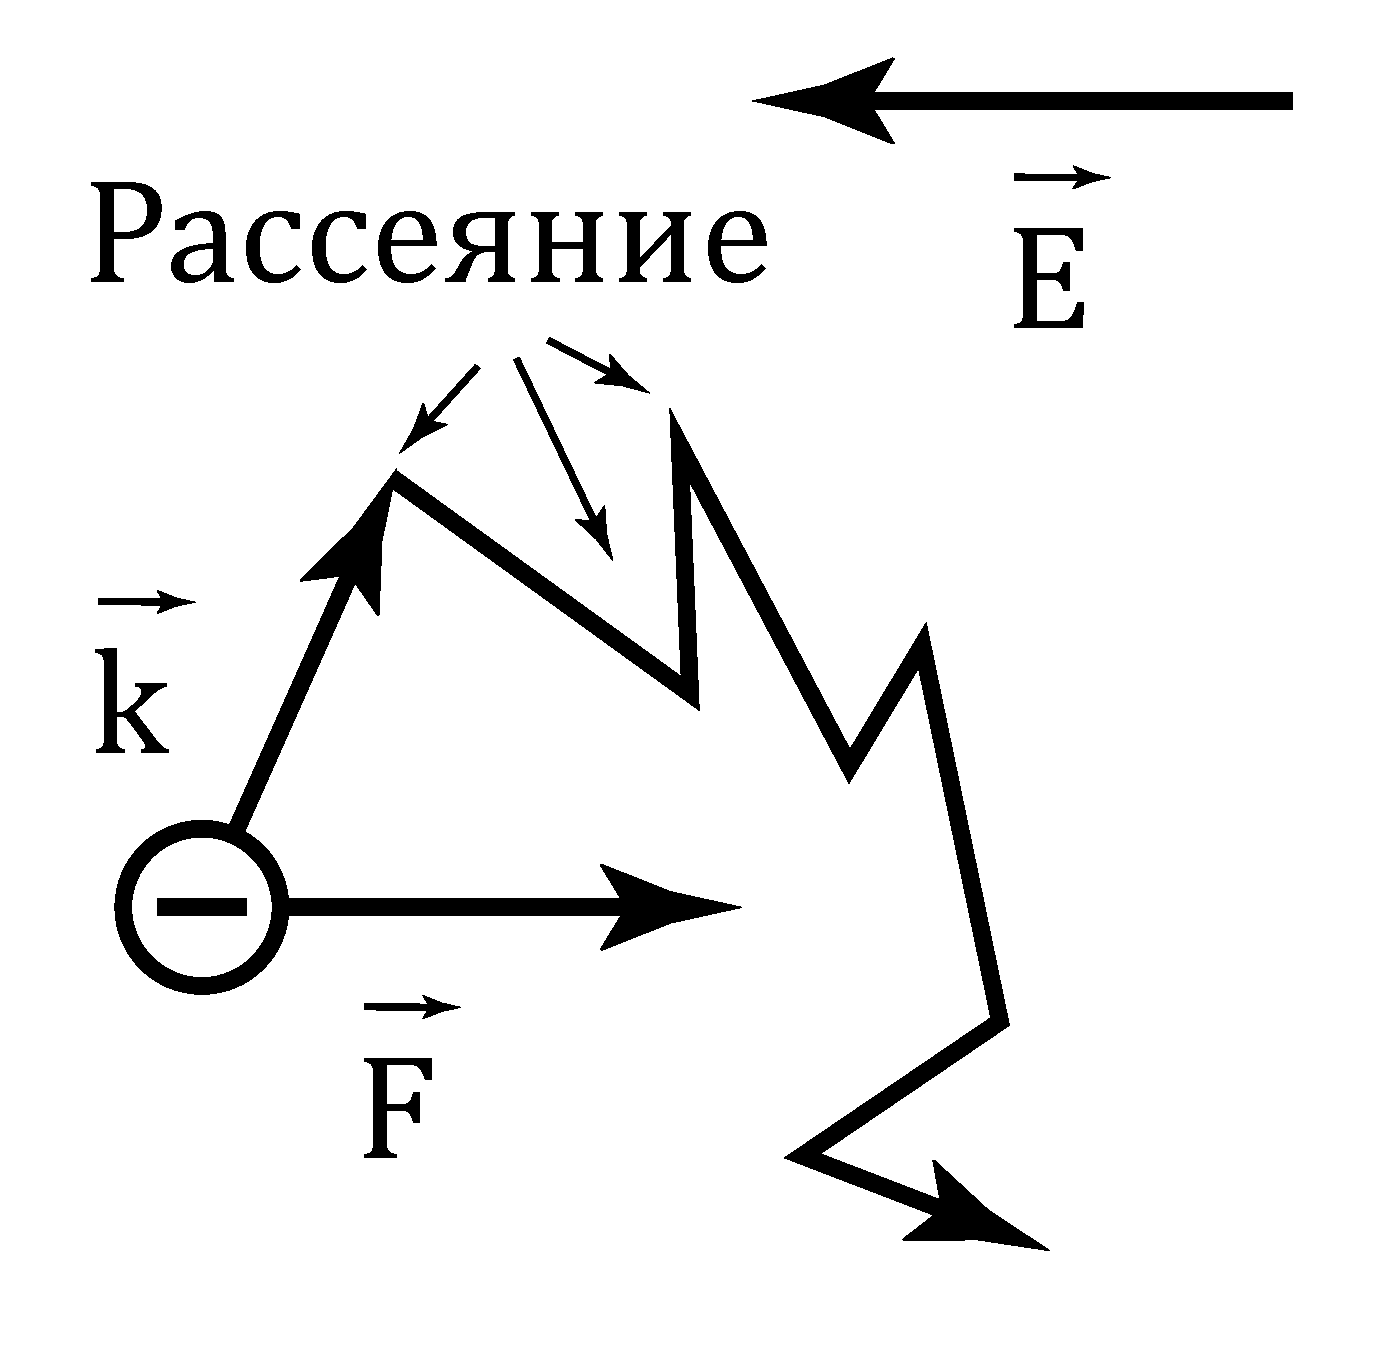
\includegraphics[width = .9\linewidth]{img/31}
			\caption{Схематическое изображение движения электрона в полупроводнике под действием электрического поля.}
			\label{fig:3.1}
		\end{wrapfigure}
		
		Электрическое поле ионизованного примесного атома распространяется на много периодов кристаллической решетки, и
		электрон, проходя на значительном расстоянии от иона, изменит под действием его поля направление своего движения. Пусть
		рассеяние в полупроводнике происходит только на ионах примеси, а тепловые колебания и нейтральные центры рассеяния
		отсутствуют. Тогда, как показывают расчеты, подвижность зависит от температуры как $T^{3/2}$, т.е. увеличивается. Этот
		результат легко понять, если учесть, что с ростом температуры увеличивается средняя скорость хаотического движения
		электронов, а быстрые электроны слабее отклоняются статическим полем ионов. Этот механизм рассеяния играет основную роль
		при температурах, когда уже имеется большая концентрация ионизированных примесей, но тепловые колебания еще мало влияют
		на рассеяние. 
		
		Рассмотрим теперь полупроводник, в котором отсутствуют примеси и дефекты, а рассеяние происходит только на тепловых
		колебаниях решетки. С ростом температуры амплитуда колебаний возрастает или, говоря языком квантовой статистики,
		возрастает концентрация фононов в кристалле. Очевидно, что рассеяние с ростом температуры должно усиливаться, а
		подвижность падать. Для неполярных полупроводников, таких как германий и кремний, уменьшение подвижности происходит по
		закону $T^{3/2}$. 
		
		Если же действует одновременно все три механизма рассеяния, то результирующая подвижность будет определяться так: 
		\begin{equation}
		\frac{1}{\mu_{\Sigma}} = \frac{1}{\mu_{1}}+\frac{1}{\mu_{2}}+\frac{1}{\mu_{3}}
		\label{eq:3.1}
		\end{equation}
		
		Поскольку подвижность – это средняя скорость в единичном электрическом поле, то она пропорциональна среднему времени
		свободного пробега $\tau$, за которое электрон набирает направленную скорость. Если $\tau_1, \tau_2,\tau_3$ – времена свободного
		пробега для каждого из трех механизмов рассеяния, то $1/\tau_1,1/\tau_2,1/\tau_3$ – соответствующие частоты столкновений. Когда
		действует несколько механизмов рассеяния, то эти частоты складываются арифметически, откуда и следует формула \eqref{eq:3.1}. Для
		выполнения данной работы важно, что итоговая зависимость подвижности от температуры является степенной функцией. 
		
		
		\begin{figure}[h!]
			\centering
			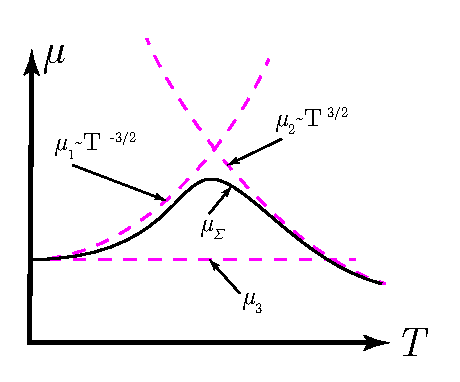
\includegraphics[width = .5\linewidth]{img/32}
			\caption{Зависимость подвижности носителей заряда в полупроводнике от температуры.}
			\label{fig:3.2}
		\end{figure}
		
		\section{Температурная зависимость проводимости}
		Плотность тока, создаваемого всеми свободными электронами, равна:
		\begin{equation}
		j=e n \mu_{n} E=\sigma_{n} E
		\label{eq:4.1}
		\end{equation}
		где n – концентрация электронов, $\sigma_n = e n \mu_n$ – удельная проводимость полупроводника, обусловленная электронами.
		Если имеется два типа носителей в полупроводнике – электроны и дырки,
		то проводимость равна:
		\begin{equation}
		\sigma=e\left(n \mu_{n}+p \mu_{p}\right)
		\label{eq:4.2}
		\end{equation}
		Для определения температурной зависимости проводимости необходимо перемножить зависимости концентрации и подвижности носителей заряда от
		температуры. При низких температурах и неполной ионизации примесей концентрация зависит от обратной температуры по экспоненциальному закону
		\eqref{eq:2.9}, а подвижность – по степенному, т.е. температурная зависимость концентрации определяет температурную зависимость проводимости:
		\begin{equation}
		\sigma=\sigma_{d} e^{\left(-\Delta W_{d} / 2 k_{B} T\right)}
		\label{eq:4.3}
		\end{equation}
		
		Здесь $\sigma_d$ содержит степенную зависимость подвижности и эффективной плотности состояний от температуры.
		
		В области истощения примесей концентрация не зависит от температуры, поэтому в этой области температурная зависимость проводимости определяется
		степенной зависимостью подвижности от температуры. И, наконец, при больших температурах зависимость проводимости от
		обратной температуры экспоненциальна, т.к. $\mu \approx T^{3/2}$, а  $N_c \approx T^{3/2}$:
		\begin{equation}
		\sigma=\sigma_{c} e^{\left(-W_{g} / 2 k_{B} T\right)}
		\label{eq:4.4}
		\end{equation}
		\begin{figure}[h!]
			\centering
			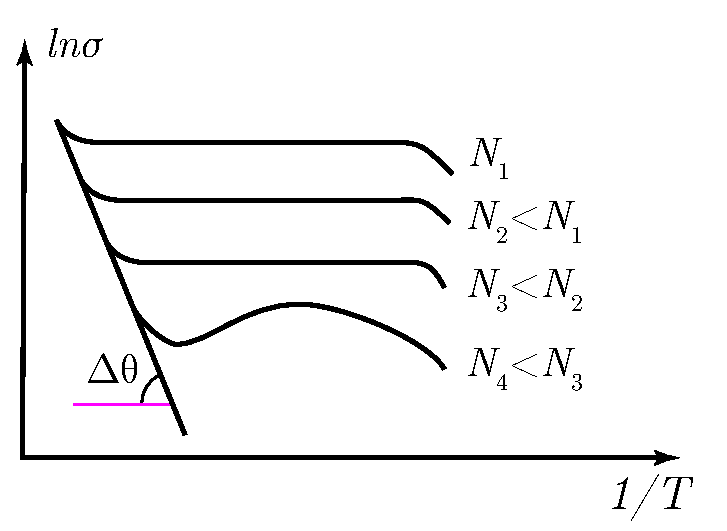
\includegraphics[width = .5\linewidth]{img/41}
			\caption{Качественный вид зависимости удельной проводимости полупроводника от температуры для различных уровней легирования (N-концентрация легирующей примеси)}
			\label{fig:4.1}
		\end{figure}
		
		На рис. \ref{fig:4.1} показана зависимость $ln(\sigma)$ от обратной температуры при различных уровнях легирования полупроводника. По
		экспериментально измеренным зависимостям $\sigma(T)$ , аналогичным рис.\ref{fig:4.1}, можно определить ширину запрещенной зоны и
		энергию активации примесей. 
		
		\section{Методика измерений}
		
		\begin{figure}[h!]
			\centering
			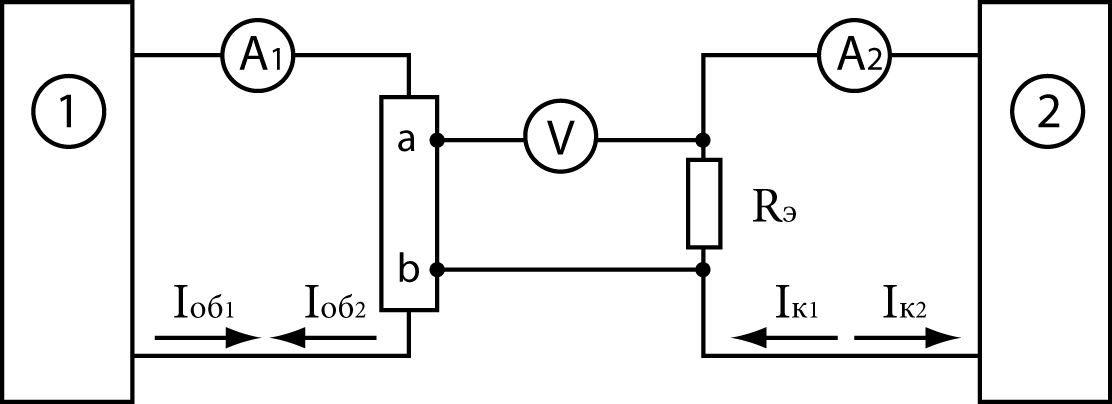
\includegraphics[width = .9\linewidth]{img/scheme.jpg}
			\caption{Электрическая схема для измерений удельной электропроводности методом компенсации}
			\label{fig:5.1}
		\end{figure}
		
		Регулируемый источник тока (1) задаёт ток образца $I_\text{об}$, измеряемый амперметром $A1$. Регулируемый источник тока
		(2) задаёт ток компенсации $I_\text{к}$ через эталонный резистор $R_\text{э}$, величина этого тока измеряется
		амперметром $А2$. Напряжение $U_{ab}$ между зондовыми электродами a и b сравнивается с напряжением компенсации $U_k$ на
		эталонном резисторе $R_\text{э}$ при помощи индикатора компенсации V.
		
		При проведении измерений нужно установить ток образца, затем, изменяя ток компенсации, добиться нулевых показаний
		индикатора компенсации V. В этом случае напряжение $U_k$ на эталонном резисторе $R_\text{э}$ будет равно напряжению $U_{ab}$:
		\begin{equation}
		U_{ab}=U_{k}=I_{k} R_{\text{э}} 
		\label{eq:5.1}
		\end{equation}
		
		В реальной ситуации между зондовыми электродами будут паразитные потенциалы, связанные, во-первых, с влиянием
		переходного сопротивления на контактах «образец – подводящие провода», во-вторых, появлением термоЭДС на контактах
		полупроводника с металлом при нагреве образца. Для того чтобы устранить влияние этих потенциалов, измерение тока
		компенсации производится дважды. Получив первый отсчёт $I_{k1}$, изменяем направление тока через образец и через
		эталонный резистор, опять добиваемся равенства напряжений $U_k$ и $U_{ab}$, снимаем второй отсчёт $I_{k2}$. Обратите
		внимание, что полярность разности потенциалов между электродами a и b, вызванная протеканием тока через образец, как и
		напряжение на $R_\text{э}$, сменились на противоположные, а паразитные потенциалы, зависящие от свойств контактов, и
		термоЭДС, зависящая от температуры образца, остались прежние. Таким образом, среднеарифметическое значение 
		
		$$I_k=\frac{I_{k1}+I_{k2}}{2}$$
		
		будет содержать информацию только о полезной составляющей напряжения $U_{ab}$.
		
		Величину падения напряжения $U_k$ легко подсчитать:
		$$U_{k}=I_{k} R_{\text{э}}$$
		
		Величину сопротивления участка образца расположенного между зондовыми электродами a и b ($R_{\text{об}}$) можно определить из равенства:
		$$R_{\text{об}}=\frac{U_{k}}{I_{\text{об}}}=\frac{I_{k} R_{\text{э}}}{I_{\text{об}}}$$
		Зная размеры образца: a - ширина (см), d - толщина (см), l - расстояние между электродами a и b (см), можно рассчитать удельное сопротивление образца:
		$$\rho=\frac{d a}{l} R_{\text{об}} (\text{Oм} \text{ cм})$$
		
		или обратную величину - удельную электропроводность: 
		$$\sigma=1 / \rho\left(\text{Oм}^{-1} \text{cм}^{-1}\right)$$
		
		\section{Схема экспериментальной установки}
		Внешний вид установки можно увидеть на рис. \ref{fig:6.1}, а её схему – на рис. \ref{fig:6.2}. 
		
		\begin{figure}[h!]
			\centering
			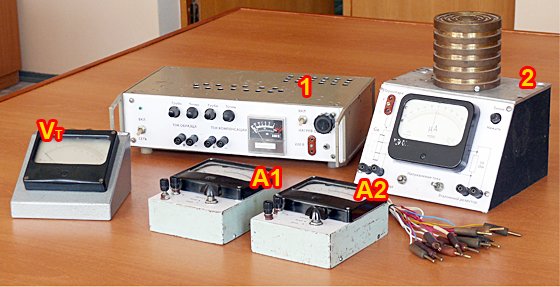
\includegraphics[width = .9\linewidth]{img/ust.jpg}
			\caption{Внешний вид установки}
			\label{fig:6.1}
		\end{figure}
		
		\begin{figure}[h!]
			\centering
			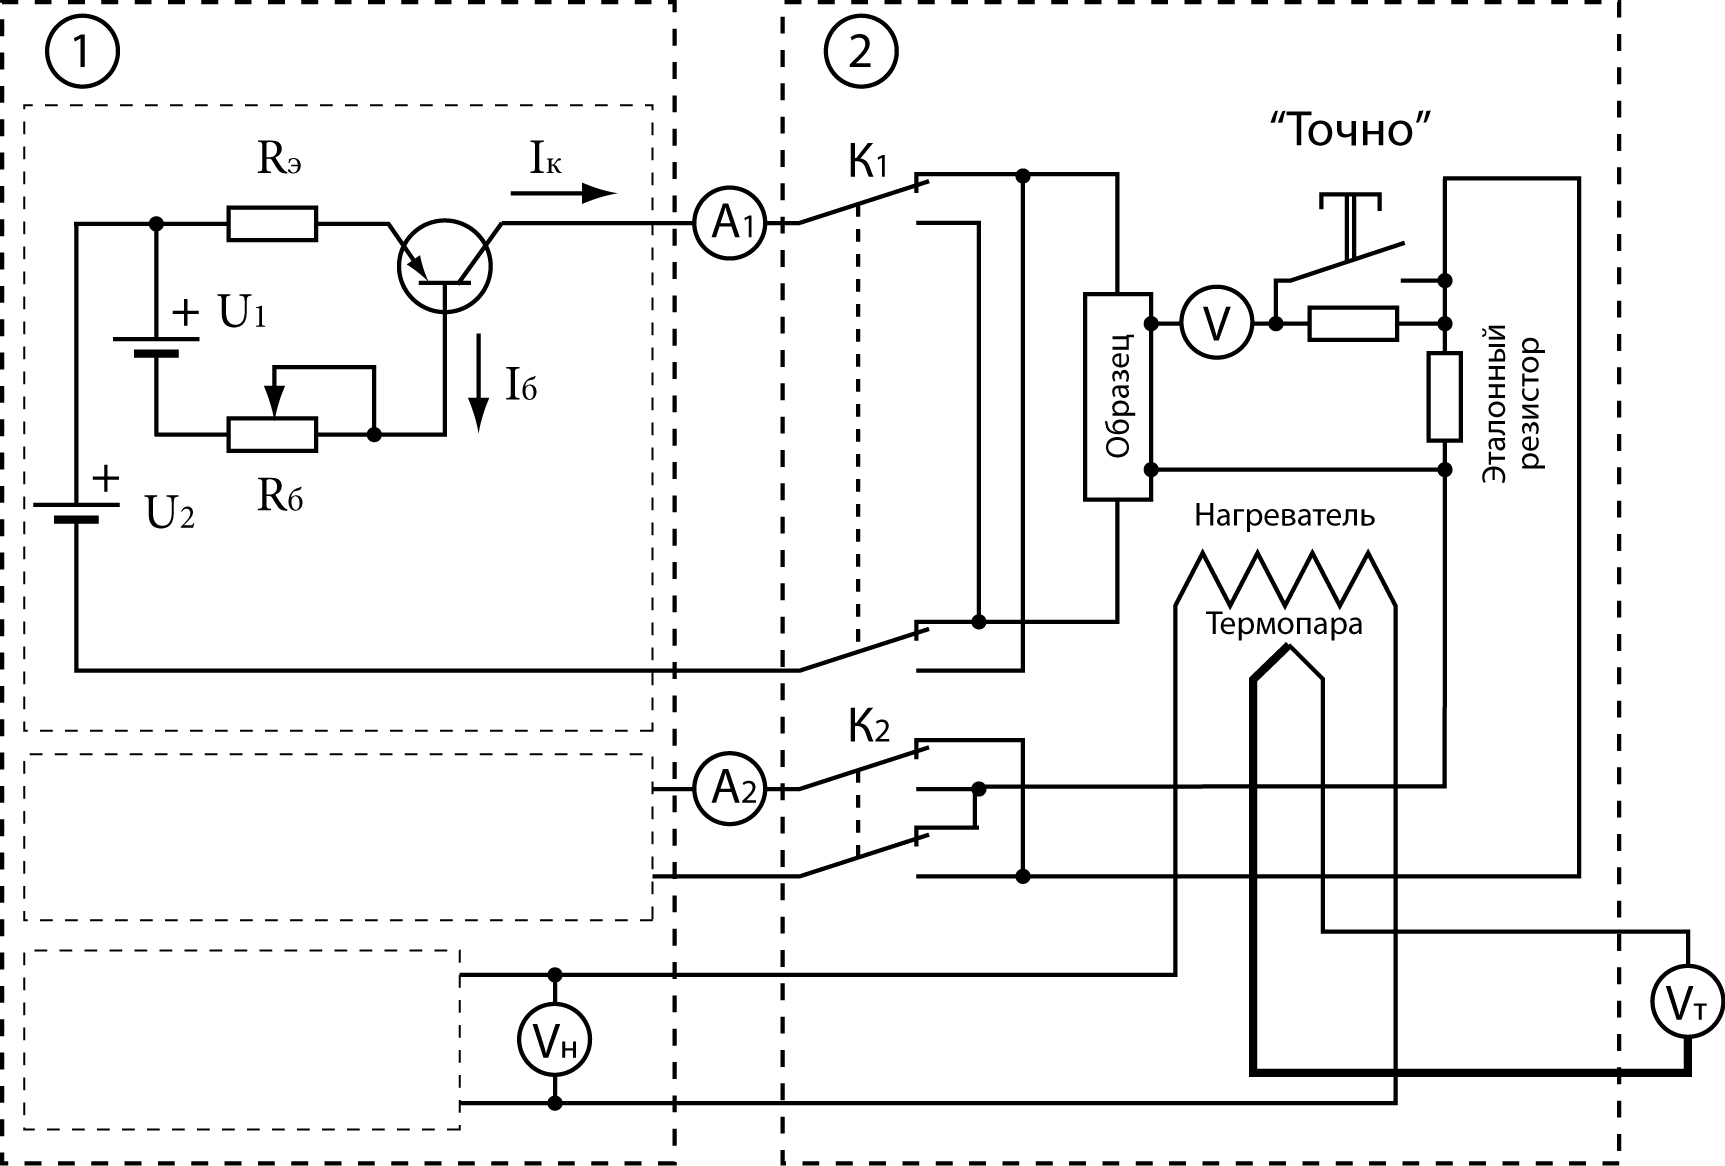
\includegraphics[width = .9\linewidth]{img/scheme-2.jpg}
			\caption{Схема установки}
			\label{fig:6.2}
		\end{figure}
		
		Блок питания (1) содержит в себе два регулируемых стабилизатора тока (для образца и эталонного резистора) и регулируемый
		источник питания нагревателя образца, напряжение на выходе которого контролируется вольтметром $V_\text{н}$. На верхней
		крышке измерительного блока (2) находится трубчатый керамический нагреватель, в котором размещён исследуемый образец и
		термопара для измерения температуры. Нагреватель с образцом и термопарой закрыты защитным цилиндром. В корпусе
		измерительного блока (2) располагается эталонный резистор Rэ, переключатели направления тока образца и компенсации К1 и
		К2, индикатор компенсации V с переключателем чувствительности «Точно». Измерение токов образца и компенсации
		производится миллиамперметрами А1 и А2 для измерения ЭДС термопары используется милливольтметр Vт, показания которого
		пересчитываются в температуру по градуировочному графику (рис. \ref{fig:6.3}).
		
		\begin{figure}[h!]
			\centering
			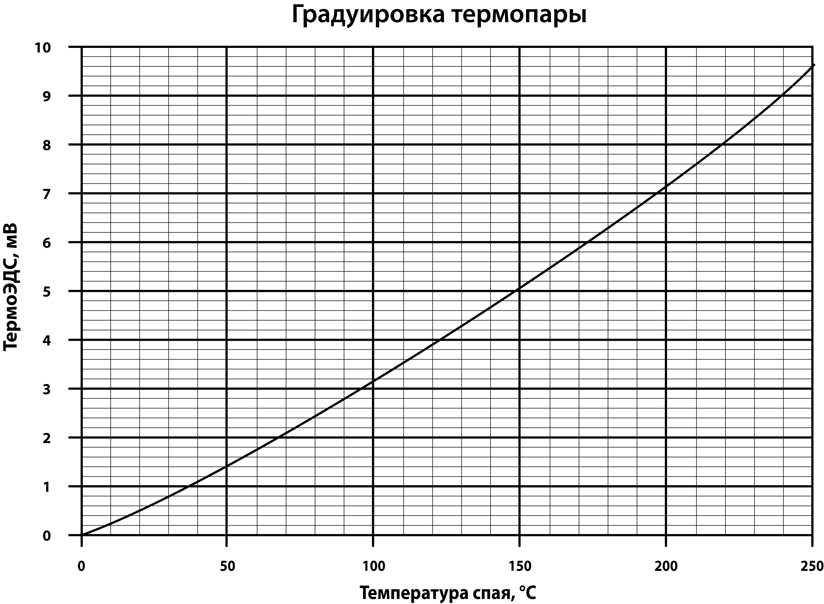
\includegraphics[width = .9\linewidth]{img/grad.jpg}
			\caption{График соответствия ЭДС термопары и температуры спая}
			\label{fig:6.3}
		\end{figure}
		
		
		\subsection{Регулируемый стабилизатор тока}
		Теоретически стабилизатор тока представляет собой источник питания с бесконечно большим выходным сопротивлением и
		бесконечно большим выходным напряжением. Не путайте его со стабилизатором напряжения, который имеет нулевое выходное
		сопротивление и может выдать бесконечно большой ток (в теории, конечно).
		
		В качестве управляющего элемента стабилизатора тока используется биполярный транзистор, включённый по схеме с общим
		эмиттером. Резистором $R_\text{б}$ можно изменять ток базы транзистора, что приведёт к изменению тока коллектора
		транзистора (от 0 до 100 мА), в цепь которого включается нагрузка (образец, эталонный резистор). В данной схеме
		определяющим является свойство транзистора поддерживать ток коллектора независимо от напряжения на коллекторе,
		естественно, в определённом диапазоне и с определённой точностью (см. рис. \ref{fig:6.4}).
		\begin{figure}[h!]
			\centering
			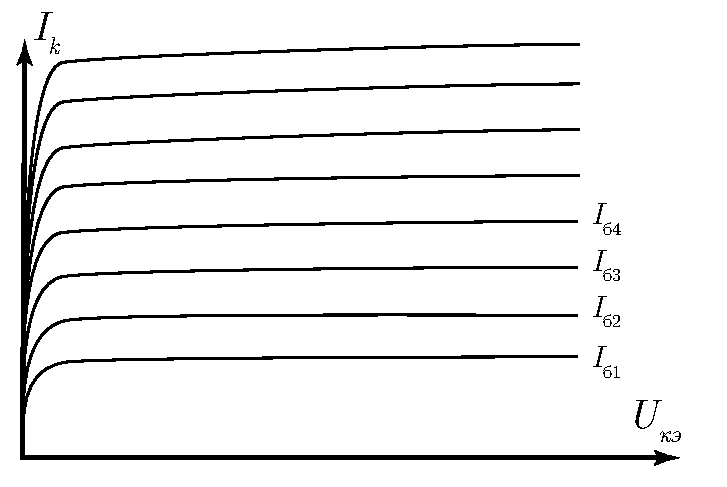
\includegraphics[width = .5\linewidth]{img/61}
			\caption{Качественный вид выходной вольтамперной характеристики биполярного транзистора, включенного по схеме с
				общим эмиттером, при различных значениях тока базы. Iк – ток коллектора, Iб – ток базы, Uкэ – напряжение между коллектором и эмиттером}
			\label{fig:6.4}
		\end{figure}
		Для увеличения стабильности значения тока служит резистор Rэ (не путайте с эталонным резистором на рис. 5.1), через
		который осуществляется отрицательная обратная связь по току: если, например, сопротивление образца уменьшится (при его
		нагреве), ток в цепи образца увеличится, что приведёт к уменьшению тока базы транзистора Iб, т. к.
		$I_\text{б} = (U_1 - R_\text{э} \cdot I_\text{к}) / (R_\text{б} + R_\text{бэ})$, где $R_\text{бэ}$ – сопротивление перехода база-эмиттер.
		
		Уменьшение тока базы уменьшит ток коллектора, а значит, и ток образца до прежней величины.
		Аналогичные по схемному решению стабилизаторы тока используются для подачи тока в цепь компенсации (на эталонный
		резистор) и на нагреватель.
		
		\subsection{Миллиамперметры А1, А2}
		Для измерения тока образца и тока компенсации в установке используется многопредельные миллиамперметры, изготовленные на
		базе серийного микроамперметра. Как пользоваться многопредельными приборами, можно прочитать на
		\href{http://www.rf.unn.ru/eledep/}{сайте} в разделе «Студентам – Инструкции».
		
		\subsection{Милливольтметр $V_T$}
		Милливольтметр используется для измерения термоЭДС термопары, установленной внутри нагревателя рядом с образцом. По
		градуировочному графику (рис. \ref{fig:6.3}) можно определить температуру спая термопары. Не забывайте, что термопары градуируются
		при температуре свободных концов 0 $^{\circ} $С.
		
		\subsection{Образец}
		Измеряемый образец изготовлен из германия, его размеры и расстояние между зондами написаны на передней панели измерительного блока.
		
		\subsection{Нагревательный элемент}
		Для нагрева образца с целью снятия зависимости его проводимости от температуры исользуется трубчатый керамический
		нагреватель, внутрь которого установлены образец и термопара. Температура нагревателя определяется величиной подаваемого
		с блока питания напряжения, которое контролируется вольтметром, находящимся на передней панели блока питания. Измерение
		температуры производится посредством термопары, расположенной внутри нагревателя в непосредственной близости от образца.
		Максимально допустимая температура образца 250 $^{\circ}$С.
		
		\subsection{Термопара}
		Термопара служит для измерения температуры образца. Её термоЭДС измеряется милливольтметром Uт и по градуировочному
		графику (рис. \ref{fig:6.3}) пересчитывается в температуру. Не забывайте, что термопары градуируются при температуре свободных
		концов 0 $^{\circ}$С.
		
		\subsection{Индикатор компенсации}
		Индикатором компенсации V является микроамперметр с нулём в середине шкалы, он показывает разность между напряжением на
		измерительных электродах образца и напряжением на эталонном резисторе. С целью расширения диапазона чувствительности
		индикатора в его цепь включен ограничительный резистор, замыкаемый кнопкой «Точно».
		
		\subsection{Переключатели направления тока}
		Переключатели К1 и К2 служат для изменения направления тока образца и тока компенсации, что необходимо для компенсации паразитных напряжений.
		
		\subsection*{Практические задания}
		
		\begin{enumerate}
			\item Произведите измерение электропроводности образца при комнатной температуре. Установив ток образца 5-10 мА
			добейтесь нулевого отклонения индикатора компенсации сначала грубой регулировкой тока компенсации, затем точной,
			нажав при этом кнопку «Точно» на передней панели измерительного блока. Проделайте это же, сменив направление тока.
			\item Проведите такие же измерения при различных температурах. Включив нагрев образца, установите напряжение
			нагревателя примерно 10\% от максимального значения. Температура устанавливается в течение 5-10 минут. Увеличивая
			напряжение нагревателя, снимите температурную зависимость тока компенсации (для двух направлений тока при каждом
			значении температуры) через 15-20 $^{\circ}$С. Максимально допустимая температура образца 250 $^{\circ}$С.
			С увеличением температуры для обеспечения удовлетворительной точности измерений потребуется увеличить ток образца.
		\end{enumerate} 


\subsection*{Обработка результатов измерений}
\begin{enumerate}
	\item Построить график полученной зависимости в координатах $ln(\sigma)-10^3/T$ (Т – абсолютная температура в градусах К).
	\item Прологарифмировать выражение \eqref{eq:4.4} и найти связь между угловым коэффициентом наклона кривой
	$ln(\sigma)-10^3/T$ и величиной $W_g$.
	\item Определить угловой коэффициент наклона кривой $ln(\sigma)-10^3/T$ в области высоких температур и рассчитать
	значение $W_g$ (в электронвольтах).
	\item В области истощения примесей определить зависимость $\sigma = f(T)$, считая, что $\sigma \approx T^n$. Ее
	можно найти, взяв на кривой две точки и воспользовавшись соотношением $\sigma_{I} / \sigma_{2}=\left(T_{I} /
	T_{2}\right)^{n}$.
	\item Определить (экстраполяцией по графику) величину $\sigma_c$, соответствующую
	электропроводности вещества при $T \to \infty$.
\end{enumerate}
\newpage
\section* {Эксперимент}
\textbf{Оборудование}
\begin{enumerate}
	\item $R{\text{э}} = 10$ Ом.
	\item Образец $l = 7$ см, $d=1.4$ см, $a = 4$ см $x = 20$ см.
\end{enumerate}

Произвели измерение электропроводности образца при комнатной температуре. Установив ток образца 5-10 мА
добились нулевого отклонения индикатора. Провели те же действия, сменив направление тока.

Такие же измерения провели при различных температурах. Сняли температурную зависимость тока компенсации (для двух направлений тока при каждом
значении температуры $I_{k1},I_{k2}$).

Далее взяли среднее значение тока:
$$I_k=\frac{I_{k1}+I_{k2}}{2}$$

Рассчитали проводимость для каждой снятой точки по формуле:

$$\sigma = \frac{l}{ad} \frac{I_{\text{об}}}{ I_k ~ R_{\text{э}}}$$

\subsection*{Задание 1}
\begin{figure}[H]
	\centering
	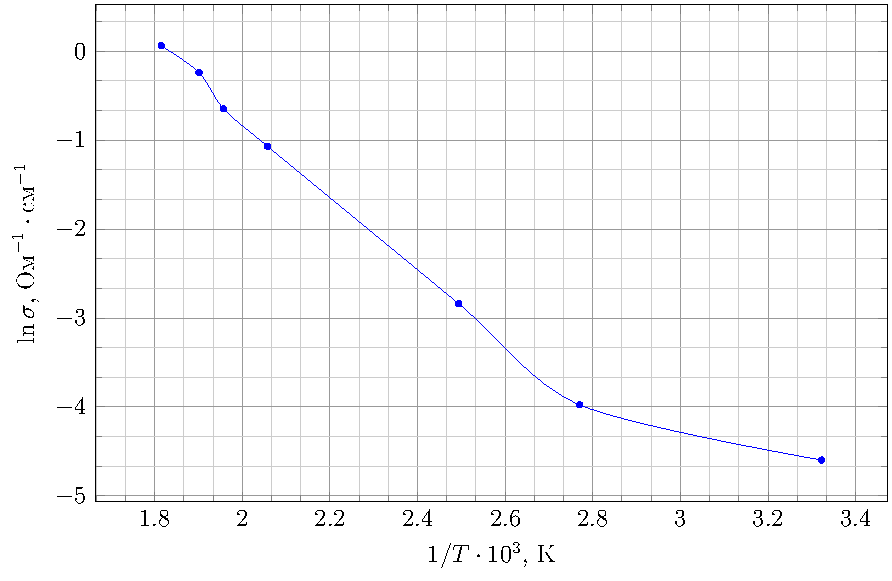
\includegraphics[width=0.8\linewidth]{plots/fig1.pdf}
	\caption{Зависимость $\sigma(T)$}
	\label{fig:exp.1}
\end{figure}

\subsection*{Задание 2}
Прологарифмировав выражение \eqref{eq:4.4} было получено следующее соотношение $\displaystyle\ln\sigma = -\frac{W_g}{2k_BT}\cdot\ln\sigma_c$. Тогда связь $W_g$ с $\tan\alpha$ выглядит следующим образом: $W_g = -1000*2k_B\cdot\tan\alpha$. %$W_g = 2*8.62\cdot10^{-5}*3298 \;\text{эВ}$.

\subsection*{Задание 3}
\begin{figure}[H]
	\centering
	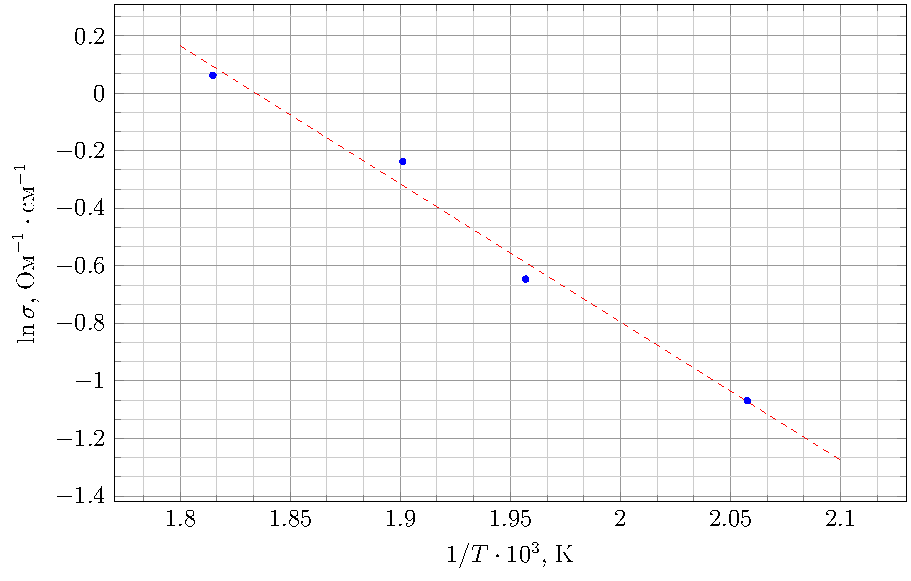
\includegraphics[width=\linewidth]{plots/fig2.pdf}
	\caption*{Зависимость $\sigma(T)$ в области высоких температур}
\end{figure}
В области высоких температур величина $W_g = 0.82 \pm 0.16\;\text{эВ}$.
\subsection*{Задание 4}
В области истощения примесей (на рис.\ref{fig:exp.1} - область значений от 2.6 до 3.4 по оси $\displaystyle(\frac{10^3}{T})$ 
определили зависимость $\sigma = f(T)$, считая, что $\sigma \approx T^n$. Ее можно найти, взяв на кривой две точки и
воспользовавшись соотношением $\sigma_{I} / \sigma_{2}=\left(T_{I} / T_{2}\right)^{n}$.

$$\ln \sigma_1 = -4.597, \ln \sigma_2 = -3.976$$
$$ T_1 = 301.15\text{ K},T_2 = 361.15 \text{ K} $$
$$ \ln \sigma_1 - \ln \sigma_2 = n \ln(\frac{T_1}{T_2})$$
$$ -4.597+3.976 = n \ln(\frac{301.15}{361.15}) $$
$$ n = 3.418 $$

\subsection*{Задание 5}
Определили (экстраполяцией по графику) величину $\sigma_c$, соответствующую
электропроводности вещества при $T \to \infty$.
$$ \ln \sigma_c = \ln \sigma (T \to \infty) \approx 8.17$$
$$\sigma_c = e^{8.17}  = 3533\text{ Ом$^{-1}$см$^{-1}$}$$
\subsection*{Контрольные вопросы}
\begin{enumerate}
	\item Что такое разрешенные и запрещенные зоны, уровень Ферми, вырожденные и невырожденные полупроводники, условие
	электронейтральности полупроводника, подвижность, плотность состояний, концентрация носителей заряда? 
	\item Что такое тип носителей заряда, собственные и примесные полупроводники? Какова энергия ионизации примесных атомов? Каковы механизмы
	рассеяния носителей заряда в полупроводниках? 
	\item Как зависят от температуры ширина запрещенной зоны, уровень Ферми, подвижность, концентрация носителей заряда, проводимость? 
	\item Методика измерения ширины запрещенной зоны. Как избежать влияния паразитной термоЭДС и контактных сопротивлений при измерениях? 
\end{enumerate}



\end{document}
